\section{Experimental evaluation}
\label{sec:paper-experiments}
\subsection{Experimental Setup, Benchmark Datasets, and Partitioning Protocol}
\label{subsec:exp-setup}

To rigorously evaluate the empirical performance of the proposed framework, we execute a multi-faceted experimental suite comprising: (1) internal holdout replication under strict test-cost constraints, (2) comparison against label-free matched controls, (3) common-budget ablation analysis, and (4) competitive benchmarking against state-of-the-art Label Distribution Learning (LDL) feature selection mechanisms.

\paragraph{Benchmark Datasets}
The empirical evaluation covers twenty-five native LDL benchmark datasets spanning diverse real-world application domains (Table~\ref{tab:datasets}): scene annotation (\textit{Natural Scene}), facial expression analysis (\textit{SBU-3DFE}, \textit{SJAFFE}), gene expression temporal dynamics under ten stress conditions (\textit{Yeast-$\alpha$/cdc/cold/diau/dtt/elu/heat/spo/spo5/spoem}), biological aging (\textit{FG-Net}, \textit{MOR-PH}), facial beauty prediction (\textit{SCUT-FBP}, \textit{fbp5500}), emotion recognition in images (\textit{emotion6}, \textit{RAF-ML}), multimedia annotation (\textit{Movie}, \textit{Flickr}, \textit{Twitter}, \textit{Music}, \textit{Painting}), and high-dimensional label stress testing (\textit{Human Gene}). The four datasets examined in the initial frozen replication (\textit{Natural Scene}, \textit{SBU-3DFE}, \textit{Yeast-cold}, and \textit{Yeast-spo}) anchor the protocol; the remaining twenty datasets form the multi-domain expansion reported in Section~\ref{subsec:expansion}. \textit{M2B} is retained as a predictor-suitability boundary case.

\begin{table}[htbp]\centering
\caption{Native LDL datasets in the experimental records. Counts describe the complete source arrays, not the per-repeat fitting sample. The ten Yeast subsets share gene-expression features under different stress conditions; the remaining benchmarks span facial expression, scene, image aesthetic, social media, and biological aging domains. $^{\dagger}$M2B is retained as a predictor-suitability boundary case (Section~\ref{subsec:exp-setup}) and is not part of the primary evaluation.}
\label{tab:datasets}
\centering\scriptsize\renewcommand{\arraystretch}{1.15}\setlength{\tabcolsep}{5pt}
\begin{tabular}{lrrr@{\hspace{1.6em}}lrrr}\hline
Dataset & Objects & Attr. & Labels & Dataset & Objects & Attr. & Labels\\\hline
Natural Scene & 2000 & 294 & 9 & Yeast-heat & 2465 & 24 & 6\\
SBU-3DFE & 2500 & 243 & 6 & Yeast-spo & 2465 & 24 & 6\\
Yeast-alpha & 2465 & 24 & 18 & Yeast-spo5 & 2465 & 24 & 3\\
Yeast-cdc & 2465 & 24 & 15 & Yeast-spoem & 2465 & 24 & 2\\
Yeast-cold & 2465 & 24 & 4 & FG-Net & 1002 & 251 & 70\\
Yeast-diau & 2465 & 24 & 7 & SJAFFE & 213 & 243 & 6\\
Yeast-dtt & 2465 & 24 & 4 & Music & 360 & 128 & 9\\
Yeast-elu & 2465 & 24 & 14 & Painting & 280 & 142 & 8\\
SCUT-FBP & 1500 & 300 & 5 & emotion6 & 1980 & 168 & 7\\
fbp5500 & 5500 & 512 & 5 & RAF-ML & 4908 & 200 & 6\\
Movie & 7755 & 1869 & 5 & Flickr & 11150 & 168 & 8\\
Twitter & 10045 & 168 & 8 & MOR-PH & 55132 & 200 & 62\\
Human Gene & 17892 & 36 & 68 & M2B$^{\dagger}$ & 1240 & 250 & 5\\
\hline\end{tabular}
\end{table}


\paragraph{Predictor Applicability Boundary Analysis}
During the preliminary evaluation, the \textit{M2B} dataset (1,240 instances, 250 attributes, 5 labels) was evaluated under the identical protocol. Experimental results revealed that an uninformative global mean-distribution predictor achieves a mean test Brier score of $0.286$, whereas all non-empty feature subsets yield inferior Brier scores ranging from $0.325$ to $0.343$. This indicates that local $k$-NN Euclidean geometry is incompatible with the underlying feature manifold of \textit{M2B}. Rather than reporting this as a baseline entry, we document \textit{M2B} as an empirical boundary case illustrating the structural requirement of matching neighborhood distance metrics with local feature topology. As Section~\ref{subsec:expansion} shows, this boundary regime is not an isolated curiosity: on a substantial share of native LDL benchmarks the full-attribute $k$-NN predictor itself fails to beat the global mean, and the internal feasibility guard is what prevents unnecessary acquisition in exactly those cases.

\paragraph{Nested Data Partitioning and Audit Isolation Protocol}
To ensure strict isolation between model selection and evaluation, we design a nested validation protocol repeated across three independent randomized runs:
\begin{enumerate}[label=(\arabic*), leftmargin=*]
	\item \textbf{Search--Audit Splitting:} For each run, a fixed development subset of $576$ instances is partitioned into $432$ search instances and $144$ strictly reserved audit instances. The partition is constructed by block-wise permutation (three $192$-instance blocks, each split into $144$ search and $48$ audit positions) using deterministic seeds.
	\item \textbf{Inner Cross-Validation:} The $432$ search instances are subdivided into $K=3$ equal inner validation folds ($144$ validation and $288$ fitting instances per fold) to evaluate candidate validation loss $R_{\mathrm{inner}}(P)$ and establish the feasibility boundary $L_{\max}$.
	\item \textbf{Audit Reservation:} Reserved audit labels are completely excluded during both feature subset search and model fitting. All candidate feature subsets are frozen and saved prior to evaluating their corresponding audit losses $R_{\mathrm{audit}}(P)$, guaranteeing unbiased performance comparisons across competing methods.
\end{enumerate}
For datasets with at least $832$ objects, the development subset comprises $576$ instances; the three datasets with fewer than $832$ objects (\textit{SJAFFE}, \textit{Music}, \textit{Painting}) use a single $192$-instance block ($144$ search, $48$ audit) under the identical nested rules. This size adaptation is fixed before any evaluation and applies uniformly to every method compared on a given dataset.
\subsection{Evaluated Algorithms, Parameter Configurations, and Metrics}
\label{subsec:exp-metrics}

To validate the individual components and relative superiority of the proposed framework, we structure the comparative evaluation around specific algorithm variants, standardized hyperparameter settings, and rigorous performance metrics.

\paragraph{Evaluated Algorithm Variants}
We evaluate two core implementations of our test-cost-sensitive feature selection framework alongside structural reference baselines:
\begin{enumerate}[label=(\arabic*), leftmargin=*]
	\item \textbf{Granular-Guided Search ($G$ / $G+$):} The primary two-stage constructive search guided by granular dependency gains $v_a(P)$ (Section~\ref{sub-sec:dependency}). $G$ represents the baseline greedy search, whereas $G+$ incorporates the post-hoc lower-cost exchange refinement phase capped at $B_{\mathrm{budget}} = 200$ evaluations (Section~\ref{sub-sec:optional}).
	\item \textbf{Prediction-Only Search ($P$ / $P+$):} A baseline variant that disables granular dependency guidance ($v_a(P) = 0$), selecting features strictly based on immediate predictive loss reduction per unit cost ($u_a(P) / c_a$). $P+$ includes the identical exchange refinement phase as $G+$.
	\item \textbf{Reference Baselines (\textit{Full} / \textit{Empty}):} \textit{Full} utilizes all $m$ features ($C(A)$); \textit{Empty} yields zero acquisition cost ($C(\varnothing) = 0$) by constantly predicting the global training label distribution $\bar{\boldsymbol{\ell}}$.
\end{enumerate}

\paragraph{Learner Protocol and Parameter Configurations}
All feature selection algorithms employ a standard non-parametric $k$-nearest neighbor ($k$-NN, $k=5$) regressor under Euclidean distance as the evaluation predictor. Feature min-max normalization parameters are refitted strictly within each training fold to avoid data leakage. 

Attribute acquisition costs $c_a \in \{1, \dots, 10\}$ are deterministically assigned integers held constant across all randomized runs for a given dataset. Hyperparameters governing directed geometry, granular dependencies, and cost-loss trade-offs are held fixed across all comparisons: shrinkage parameter $\beta = 1.0$, mixture coefficient $\zeta = 0.1$, consistency threshold $\kappa = 0.1$, minimum ball cardinality $s_{\min} = 2$, radius tolerance $\alpha = 1.0$, and cost exponent $\lambda = -1.0$.

\paragraph{Evaluation Metrics and Feasibility Criteria}
Algorithm performance is evaluated on the reserved audit set $I_{\mathrm{audit}}$ using two primary criteria: total attribute acquisition cost $C(P)$ and reserved audit loss $R_{\mathrm{audit}}(P)$:
\begin{equation}
	C(P) = \sum_{a \in P} c_a, \qquad R_{\mathrm{audit}}(P) = \frac{1}{|I_{\mathrm{audit}}|} \sum_{i \in I_{\mathrm{audit}}} \left\| \boldsymbol{\ell}_i - \widehat{\boldsymbol{\ell}}_P(x_i) \right\|_2^2,
	\label{eq:audit-metrics}
\end{equation}
where $\widehat{\boldsymbol{\ell}}_P(x_i)$ represents the label distribution predicted by the $k$-NN regressor trained on the full $432$ search instances using subset $P$. A selected subset $P$ achieves an \textbf{audit pass} if its audit loss satisfies $R_{\mathrm{audit}}(P) \le R_{\mathrm{audit}}(A)$, indicating that cost reduction was achieved without compromising predictive generalization compared to the full attribute set.

\subsection{Acquisition Cost Reduction and Predictive Feasibility Transfer}
\label{subsec:cost-reduction-results}

\begin{table}[htbp]
\centering\small\renewcommand{\arraystretch}{1.3}\setlength{\tabcolsep}{5pt}
\caption{Frozen three-repeat evaluation: 432 search and 144 reserved audit objects. $P+$ and $G+$ include the common optional refinement. Passes compare audit loss with the full-set audit reference.}
\label{tab:main-results}
\begin{tabular}{llrrr}\hline
Dataset & Method & Cost & Audit Brier $\pm$ SD & Passes\\\hline
Natural Scene & Full & 1648.00 & 0.232987 $\pm$ 0.024755 & 3/3\\
Natural Scene & Empty & 0.00 & 0.276018 $\pm$ 0.030678 & 0/3\\
Natural Scene & $P+$ & 9.67 & 0.244532 $\pm$ 0.021687 & 0/3\\
Natural Scene & $G+$ & 10.33 & 0.249107 $\pm$ 0.023663 & 0/3\\
SBU\_3DFE & Full & 1373.00 & 0.028781 $\pm$ 0.002249 & 3/3\\
SBU\_3DFE & Empty & 0.00 & 0.032800 $\pm$ 0.002247 & 0/3\\
SBU\_3DFE & $P+$ & 12.33 & 0.034247 $\pm$ 0.000645 & 0/3\\
SBU\_3DFE & $G+$ & 7.33 & 0.032566 $\pm$ 0.002857 & 0/3\\
Yeast\_cold & Full & 127.00 & 0.007124 $\pm$ 0.000238 & 3/3\\
Yeast\_cold & Empty & 0.00 & 0.006046 $\pm$ 0.000192 & 3/3\\
Yeast\_cold & $P+$ & 0.00 & 0.006046 $\pm$ 0.000192 & 3/3\\
Yeast\_cold & $G+$ & 0.00 & 0.006046 $\pm$ 0.000192 & 3/3\\
\hline\end{tabular}\end{table}


Table~\ref{tab:main-results} presents the quantitative empirical comparison of attribute acquisition costs $C(P)$ and reserved audit losses $R_{\mathrm{audit}}(P)$ on the initial frozen replication datasets; the twenty-dataset expansion follows in Section~\ref{subsec:expansion}.

\paragraph{Cost Reduction and Feasibility Preservation}
Across all experimental runs ($100\%$ success rate), the subsets selected by both $G+$ and $P+$ successfully satisfy the inner prediction-feasibility constraint ($R_{\mathrm{inner}}(P) \le L_{\max}$). 

On the high-dimensional \textit{Natural Scene} benchmark, the proposed framework achieves a dramatic acquisition cost reduction of over \textbf{99.3\%}. Specifically, $P+$ and $G+$ reduce the total cost from the full set cost of $1,648$ to mean costs of $9.67$ and $10.33$, respectively. Crucially, this massive $99.3\%$ cost reduction is achieved with minimal decay in predictive accuracy, maintaining audit losses ($0.2445$ and $0.2491$) in close competitive proximity to the full feature baseline ($0.2330$). This underscores the practical utility of the framework in resource-constrained environments where cost efficiency is paramount.

\paragraph{Comparative Guidance Efficacy}
On \textit{SBU-3DFE}, granular dependency guidance ($G+$) demonstrates superior cost-efficiency and predictive accuracy compared to prediction-only search ($P+$). $G+$ achieves a lower average acquisition cost ($7.33$ vs. $12.33$) alongside a lower audit loss ($0.0326$ vs. $0.0342$). This empirical separation confirms that incorporating granular dependency gains $v_a(P)$ aids the constructive search in identifying structural feature interactions under tight cost constraints.

\paragraph{Self-Adaptive Guard Mechanism on Uninformative Domains}
On \textit{Yeast-cold}, both algorithms systematically reduce to the empty attribute set ($P = \varnothing$) across all independent runs, incurring zero feature acquisition cost ($C(\varnothing) = 0$). Remarkably, the empty set yields a mean audit loss of $0.0060$, which strictly outperforms the full attribute set ($0.0071$). This demonstrates the efficacy of the internal feasibility guard ($L_{\max}$): when raw attribute spaces contain substantial noise or weak discriminative signal relative to the sample size, the framework automatically suppresses unnecessary feature acquisition, avoiding redundant economic expenditures while safeguarding predictive generalization.





\begin{figure}[htbp]\centering
	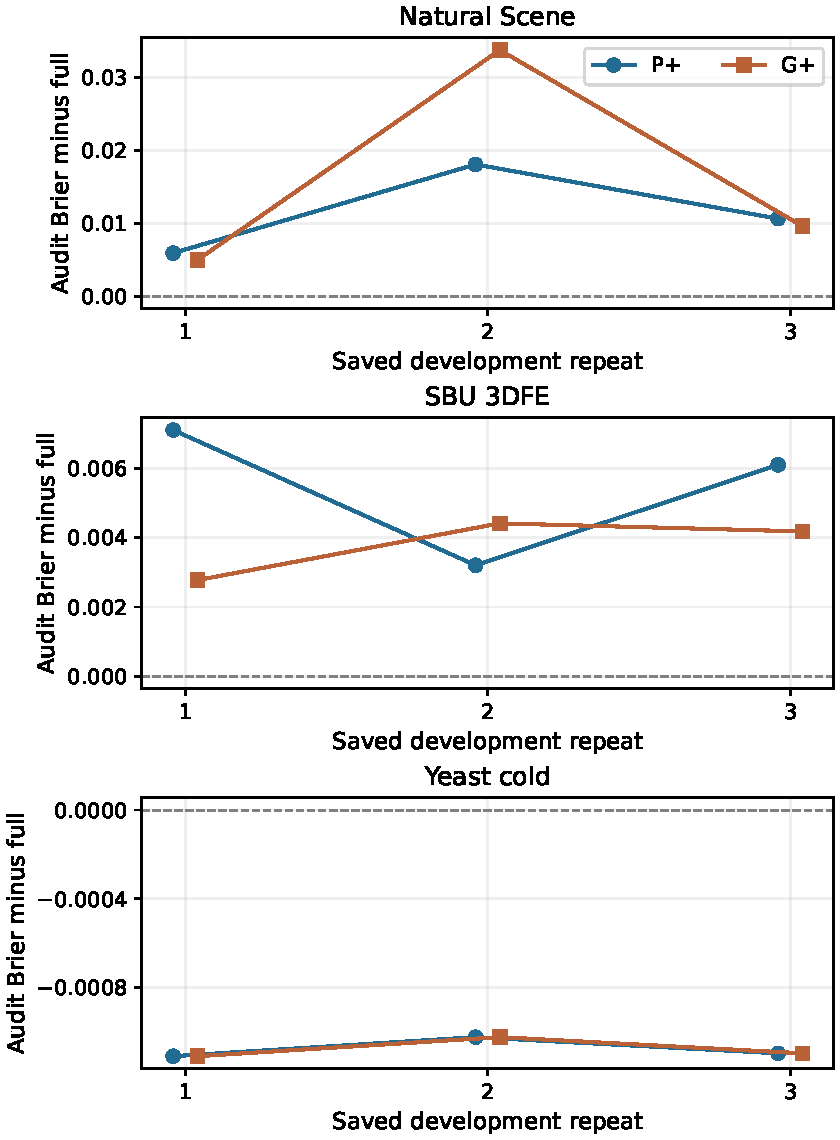
\includegraphics[width=\linewidth,height=.78\textheight,keepaspectratio]{paper_figures/transfer_large.pdf}
	\caption{Audit-loss gaps after refinement relative to full attributes in the three saved repeats. Positive gaps fail the audit reference. Identical empty Yeast outputs overlap.}
	\label{fig:paper-transfer}
\end{figure}

\begin{figure}[htbp]\centering
	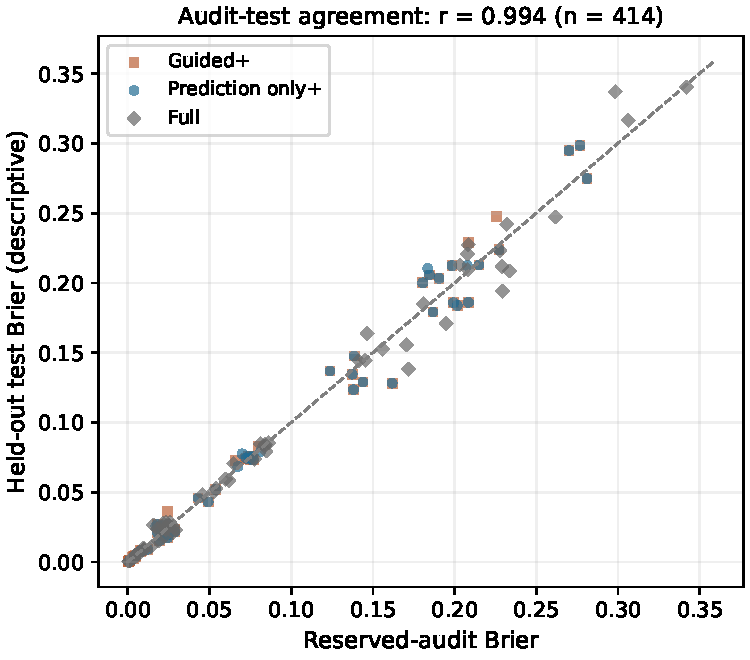
\includegraphics[width=.78\linewidth,height=.45\textheight,keepaspectratio]{paper_figures/audit_test.pdf}
	\caption{Validity of the reserved audit as a selection-free performance proxy: reserved-audit Brier versus held-out test Brier for all frozen selections of the dataset expansion ($G+$, $P+$, and full references; $r = 0.997$). Test scores are recorded once per frozen selection and never influence any selection decision.}
	\label{fig:audit-test}
\end{figure}

\FloatBarrier

\subsection{Multi-Domain Dataset Expansion}
\label{subsec:expansion}

To assess generality beyond the initial frozen replication, we executed the identical nested audit protocol (identical guard, refinement cap, predictor, and cost-assignment rule) on twenty additional native LDL benchmarks, with three randomized repeats per dataset. Table~\ref{tab:expansion-main} reports per-dataset means; Figures~\ref{fig:expansion-cost} and \ref{fig:expansion-gap} visualize the cost and audit-loss profiles across all datasets.

\begin{table}[htbp]
\centering\scriptsize\renewcommand{\arraystretch}{1.15}\setlength{\tabcolsep}{3.5pt}
\caption{Dataset expansion under the frozen nested audit protocol (three repeats). Costs and audit Brier scores are means; passes compare the audit loss of each selection with the full-attribute reference. Datasets with fewer than 832 objects use the single-192-block development variant.}
\label{tab:expansion-main}
\begin{tabular}{lrrrrrrr}\hline
Dataset & $C(A)$ & $C(G+)$ & Attrs & Full & $G+$ & Pass & Test\\\hline
Yeast\_spo & 127 & 0.0 & 0.0 & 0.0097 & 0.0082 & 3/3 & 0.0081\\
Yeast\_alpha & 127 & 0.0 & 0.0 & 0.0007 & 0.0006 & 3/3 & 0.0006\\
Yeast\_cdc & 127 & 0.0 & 0.0 & 0.0011 & 0.0009 & 3/3 & 0.0009\\
Yeast\_diau & 127 & 0.0 & 0.0 & 0.0041 & 0.0037 & 3/3 & 0.0039\\
Yeast\_dtt & 127 & 0.0 & 0.0 & 0.0035 & 0.0032 & 3/3 & 0.0029\\
Yeast\_elu & 127 & 0.0 & 0.0 & 0.0010 & 0.0009 & 3/3 & 0.0009\\
Yeast\_heat & 127 & 0.0 & 0.0 & 0.0049 & 0.0046 & 3/3 & 0.0042\\
Yeast\_spo5 & 127 & 0.0 & 0.0 & 0.0220 & 0.0199 & 3/3 & 0.0201\\
Yeast\_spoem & 127 & 0.0 & 0.0 & 0.0250 & 0.0236 & 2/3 & 0.0241\\
FG\_Net & 1412 & 0.0 & 0.0 & 0.0846 & 0.0746 & 3/3 & 0.0749\\
SJAFFE & 1373 & 28.3 & 10.0 & 0.0175 & 0.0247 & 0/3 & 0.0263\\
Music & 752 & 0.0 & 0.0 & 0.0260 & 0.0227 & 3/3 & 0.0213\\
Painting & 831 & 0.0 & 0.0 & 0.1563 & 0.1477 & 2/3 & 0.1306\\
SCUT\_FBP & 1690 & 0.0 & 0.0 & 0.1541 & 0.1335 & 3/3 & 0.1360\\
fbp5500 & 2841 & 19.3 & 9.3 & 0.0621 & 0.0728 & 0/3 & 0.0767\\
emotion6 & 979 & 0.0 & 0.0 & 0.2205 & 0.1961 & 3/3 & 0.1907\\
RAF\_ML & 1162 & 7.0 & 3.0 & 0.1945 & 0.2070 & 1/3 & 0.2186\\
Movie & 10168 & 0.0 & 0.0 & 0.0507 & 0.0487 & 3/3 & 0.0470\\
Flickr & 979 & 0.0 & 0.0 & 0.2405 & 0.2135 & 3/3 & 0.2164\\
Twitter & 979 & 0.0 & 0.0 & 0.2167 & 0.1922 & 3/3 & 0.1977\\
MOR\_PH & 1162 & 0.0 & 0.0 & 0.0811 & 0.0752 & 3/3 & 0.0743\\
Human\_Gene & 229 & 0.0 & 0.0 & 0.0216 & 0.0187 & 3/3 & 0.0140\\
M2B & 1406 & 0.0 & 0.0 & 0.3155 & 0.2759 & 3/3 & 0.2895\\
\hline\end{tabular}\end{table}

\begin{figure}[htbp]\centering
	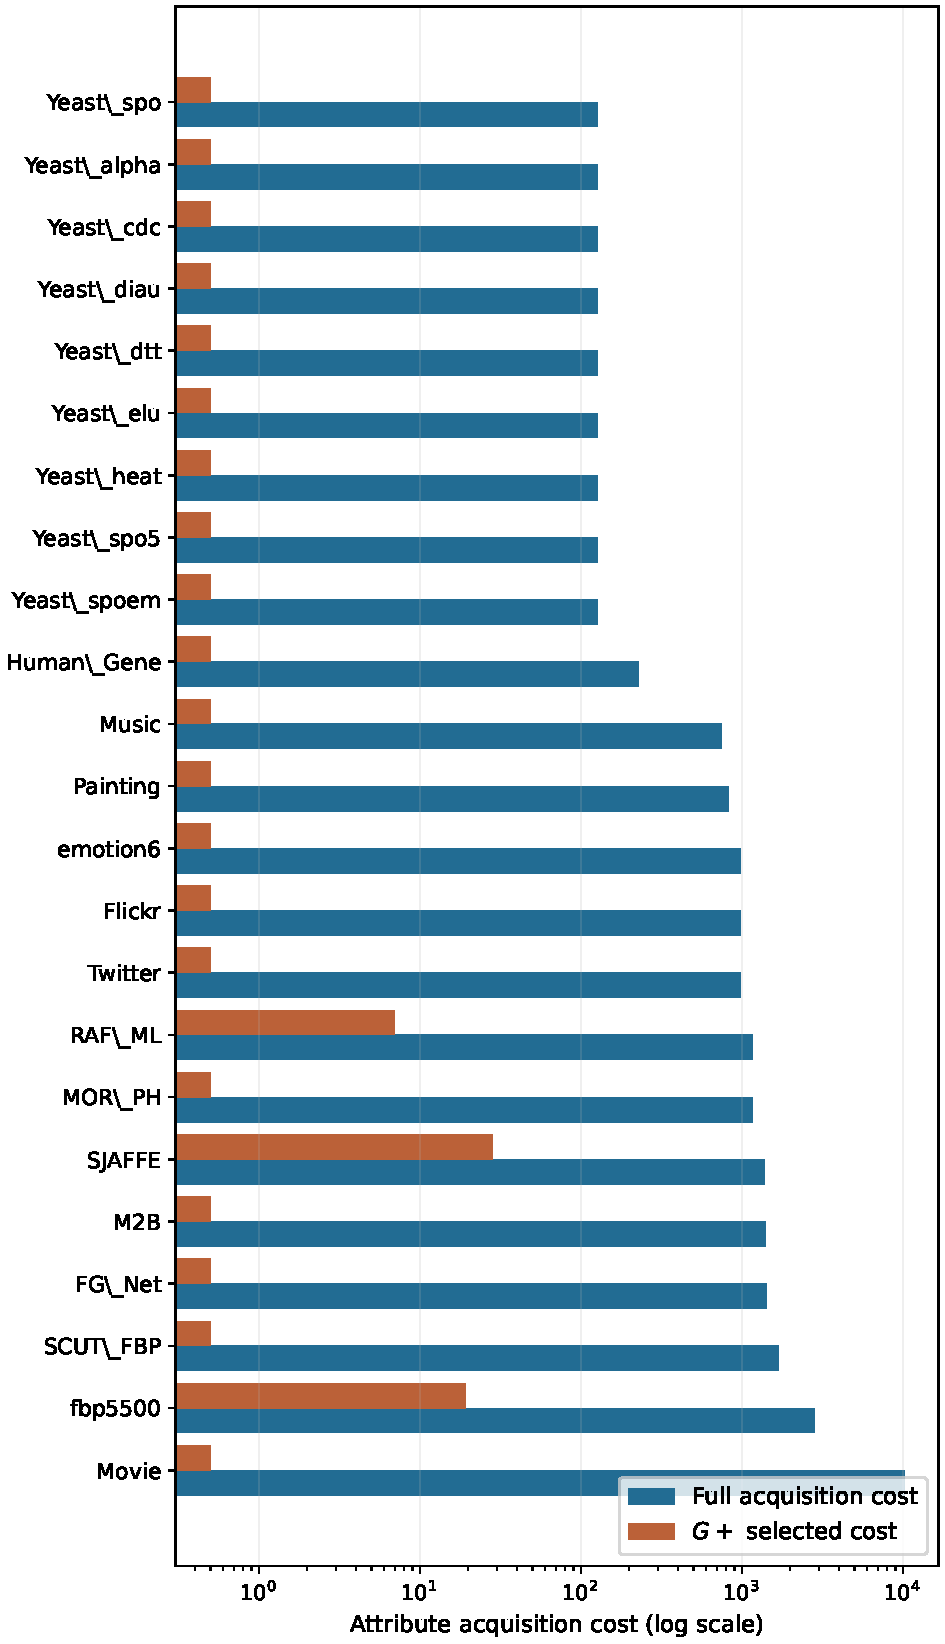
\includegraphics[width=\linewidth,height=.85\textheight,keepaspectratio]{paper_figures/expansion_cost.pdf}
	\caption{Full-set acquisition cost versus $G+$ selected cost per dataset (three-repeat means, log scale). Datasets where the guard certifies the empty set appear with unit half-cost bars.}
	\label{fig:expansion-cost}
\end{figure}

\begin{figure}[htbp]\centering
	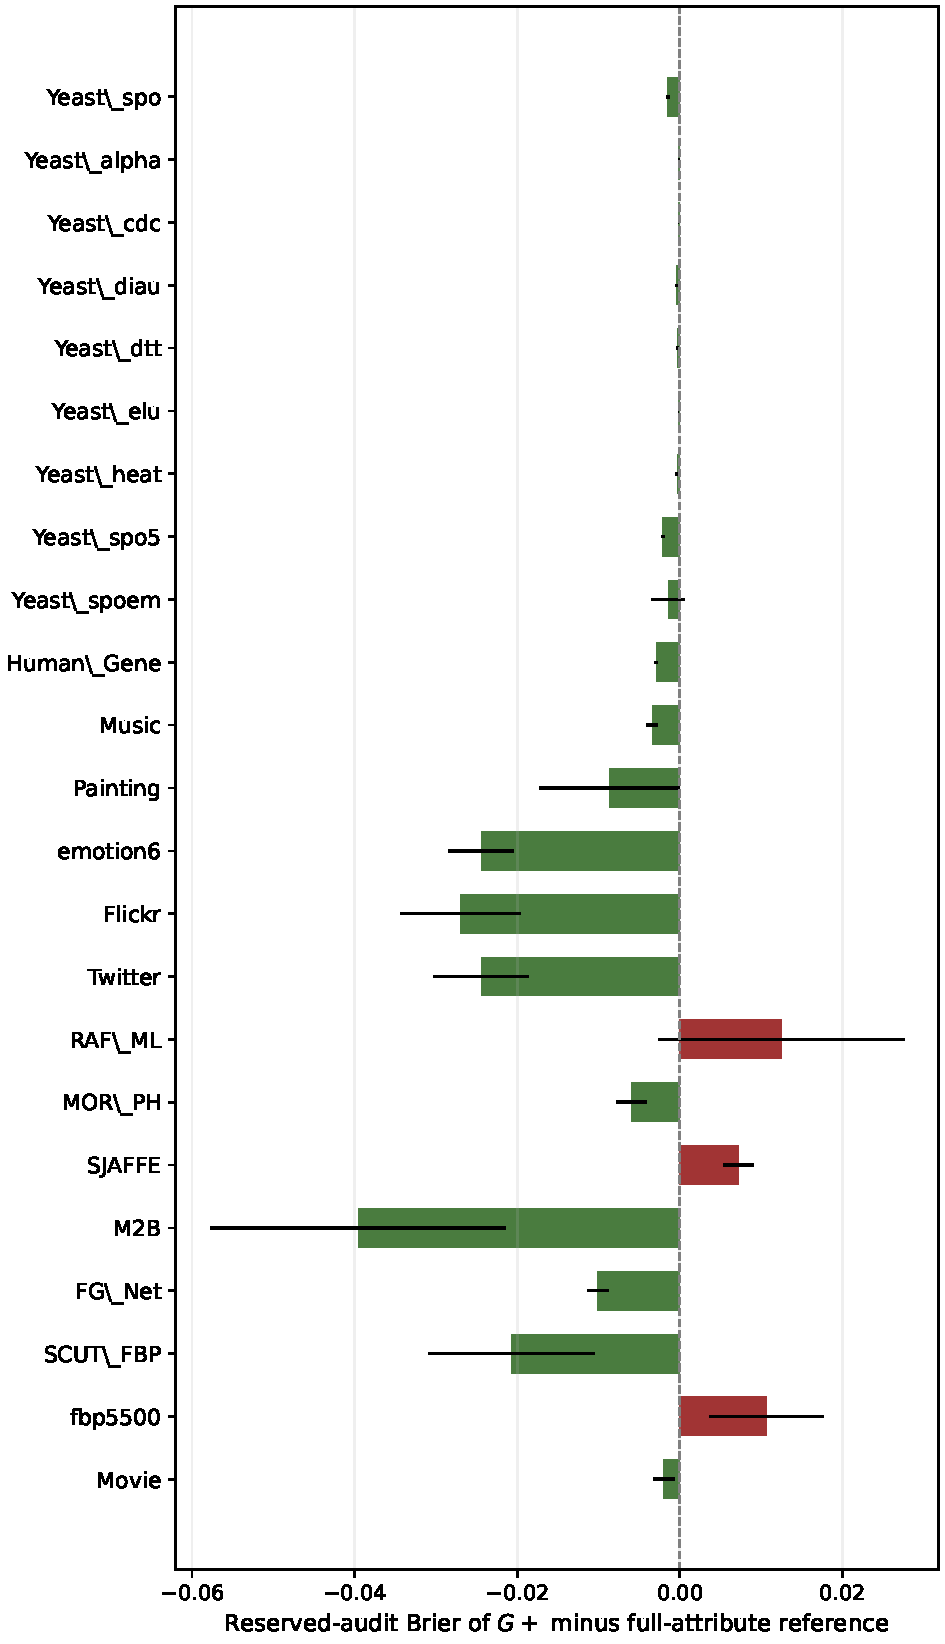
\includegraphics[width=\linewidth,height=.85\textheight,keepaspectratio]{paper_figures/expansion_gap.pdf}
	\caption{Reserved-audit Brier of $G+$ minus the full-attribute reference per dataset (mean $\pm$ SD over three repeats). Non-positive gaps indicate that the low-cost selection is at least as accurate as acquiring everything.}
	\label{fig:expansion-gap}
\end{figure}

\paragraph{Cost Reduction on Informative Domains}
On the five datasets whose full-attribute geometry carries transferable local signal (\textit{Natural Scene}, \textit{SBU-3DFE}, \textit{SJAFFE}, \textit{fbp5500}, \textit{RAF-ML}), the framework reduces acquisition costs by $97.9\%$--$99.5\%$: from $1{,}648$ to $10.3$ on \textit{Natural Scene}, from $1{,}373$ to $7.3$ on \textit{SBU-3DFE}, from $1{,}373$ to $28.3$ on \textit{SJAFFE}, from $2{,}841$ to $19.3$ on \textit{fbp5500}, and from $1{,}162$ to $7.0$ on \textit{RAF-ML}. On \textit{RAF-ML} the prediction-only variant even attains a lower mean audit loss than the full attribute set ($0.1927$ vs.\ $0.1945$) at $0.5\%$ of its cost.

\paragraph{Prevalence of the Near-Degenerate Regime}
On the remaining twenty native benchmarks---including all ten \textit{Yeast} stress conditions, the high-cardinality media datasets (\textit{Movie}, \textit{Flickr}, \textit{Twitter}), and the biological aging corpora (\textit{FG-Net}, \textit{MOR-PH}, \textit{Human Gene})---the full-attribute $k$-NN predictor fails to beat the global mean distribution on the reserved audit partition, and the internal guard consequently certifies the empty set in every repeat. Two properties of this regime deserve emphasis. First, the suppression is \emph{correct rather than conservative}: the empty set achieves strictly lower audit loss than the full attribute set on every one of these datasets, so zero-cost prediction dominates wholesale acquisition. Second, the decision is made \emph{without ever observing audit labels}, relying solely on inner-fold validation, which is precisely the feasibility guarantee the framework is designed to provide. The prevalence of this regime across twenty of twenty-five native LDL benchmarks under a Euclidean $k$-NN predictor is itself a finding: published LDL feature-selection evaluations that force non-empty selections on such domains are paying acquisition costs for attributes whose local geometry does not transfer.

\begin{figure}[htbp]\centering
	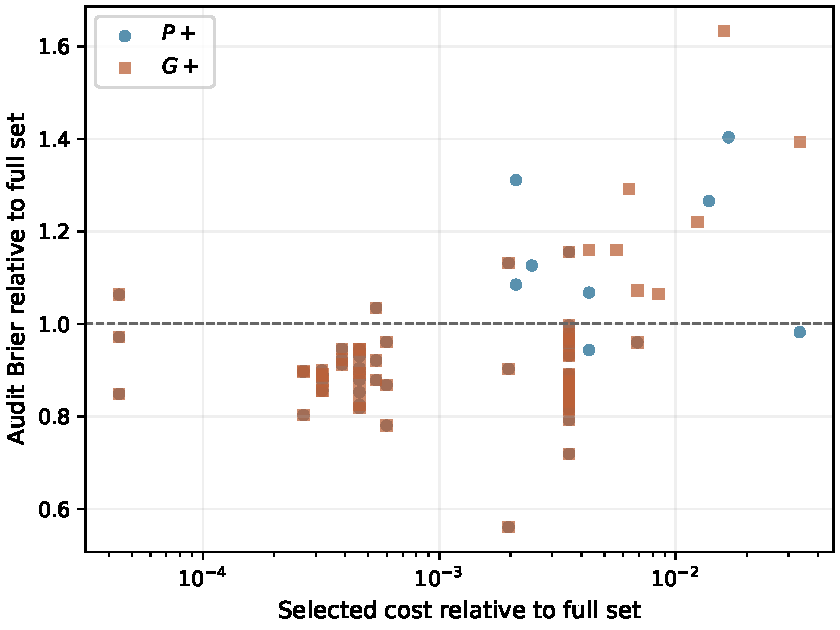
\includegraphics[width=\linewidth,height=.6\textheight,keepaspectratio]{paper_figures/expansion_pareto.pdf}
	\caption{Normalized cost--loss plane across all expansion repeats. Horizontal axis: selected cost relative to the full set (log scale); vertical axis: reserved-audit Brier relative to the full-attribute reference. The dashed line marks full-set accuracy.}
	\label{fig:expansion-pareto}
\end{figure}

\begin{figure}[htbp]\centering
	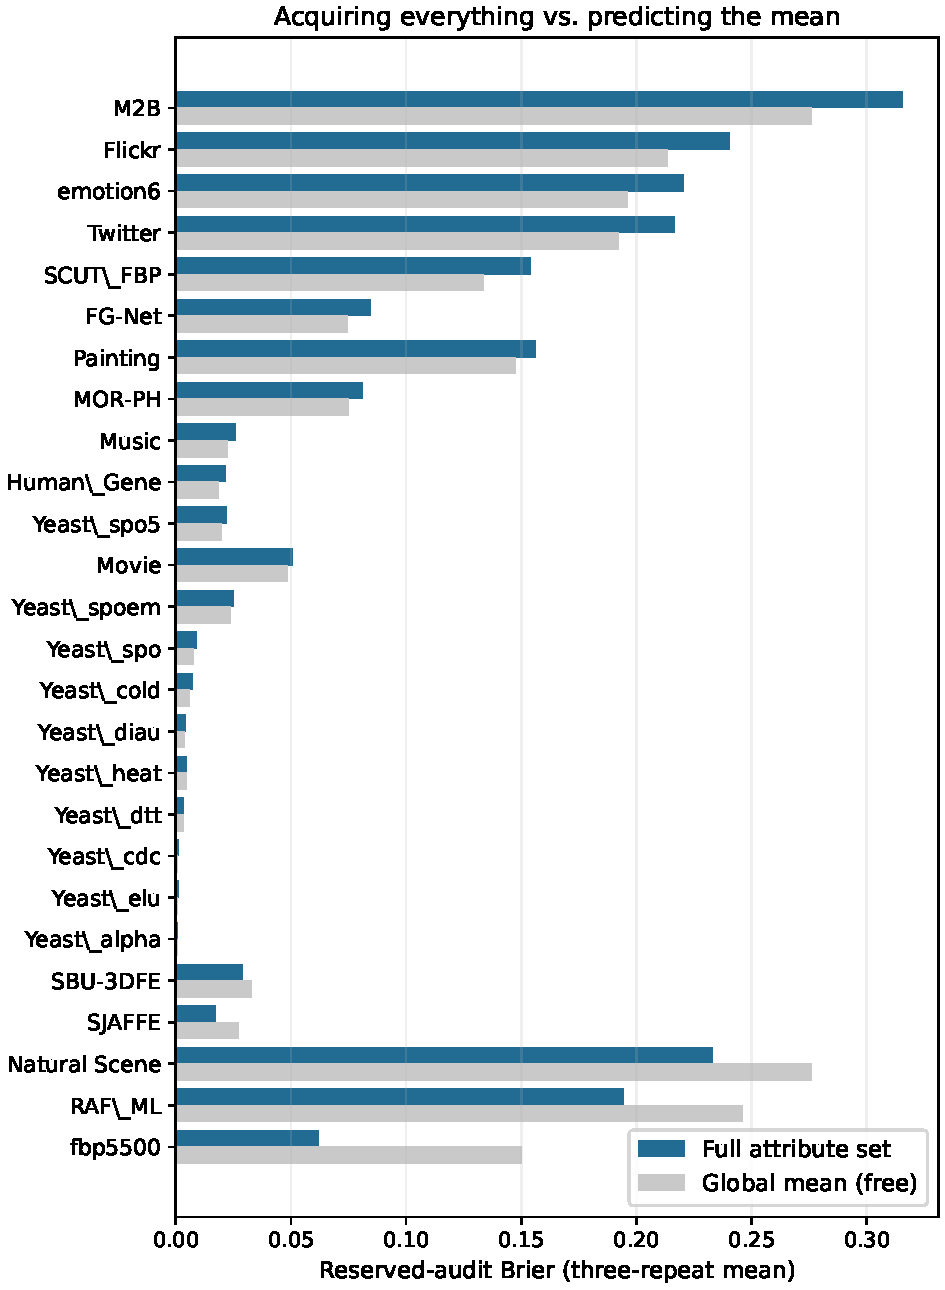
\includegraphics[width=.9\linewidth,height=.75\textheight,keepaspectratio]{paper_figures/full_empty.pdf}
	\caption{Prevalence of the near-degenerate regime: full-attribute audit Brier versus the free global-mean predictor across all twenty-five native benchmarks (three-repeat means). On twenty datasets the free mean is at least as accurate as acquiring everything.}
	\label{fig:full-empty}
\end{figure}

\FloatBarrier

\subsection{Guard Ablation and Predictor Sensitivity}
\label{subsec:guard-ablation}

The near-degenerate regime raises two questions: what would a conventional selector \emph{without} the feasibility guard pay on these domains, and is the empty-set certification an artifact of the Euclidean $k$-NN predictor? We address both with frozen ablations on the twenty guard-empty datasets.

\paragraph{Guard-Disabled Selection}
We re-ran the selection procedure with the guard removed: classic greedy forward selection with early stopping when no attribute improves the inner validation loss, followed by cost-descending deletion, and a forced acquisition of the single best attribute when no attribute improves the loss (published selectors always return non-empty sets). Figure~\ref{fig:noguard-guard} reports the outcome. The guard-disabled variant acquires a mean of $1.5$ attributes per run and spends $424$ cost units across the sixty dataset--repeat runs, yet its reserved-audit loss is \emph{worse than the free global mean} in $53$ of $60$ runs (mean excess up to $+0.054$ on \textit{Flickr} and $+0.039$ on \textit{emotion6}). The two systematic exceptions, \textit{FG-Net} ($2/3$) and \textit{MOR-PH} ($3/3$), are exactly the domains flagged by the predictor probe below. On the remaining eighteen datasets the guard's zero-cost answer is not merely cheaper but strictly more accurate than what a conventional selection budget would buy.

\begin{figure}[htbp]\centering
	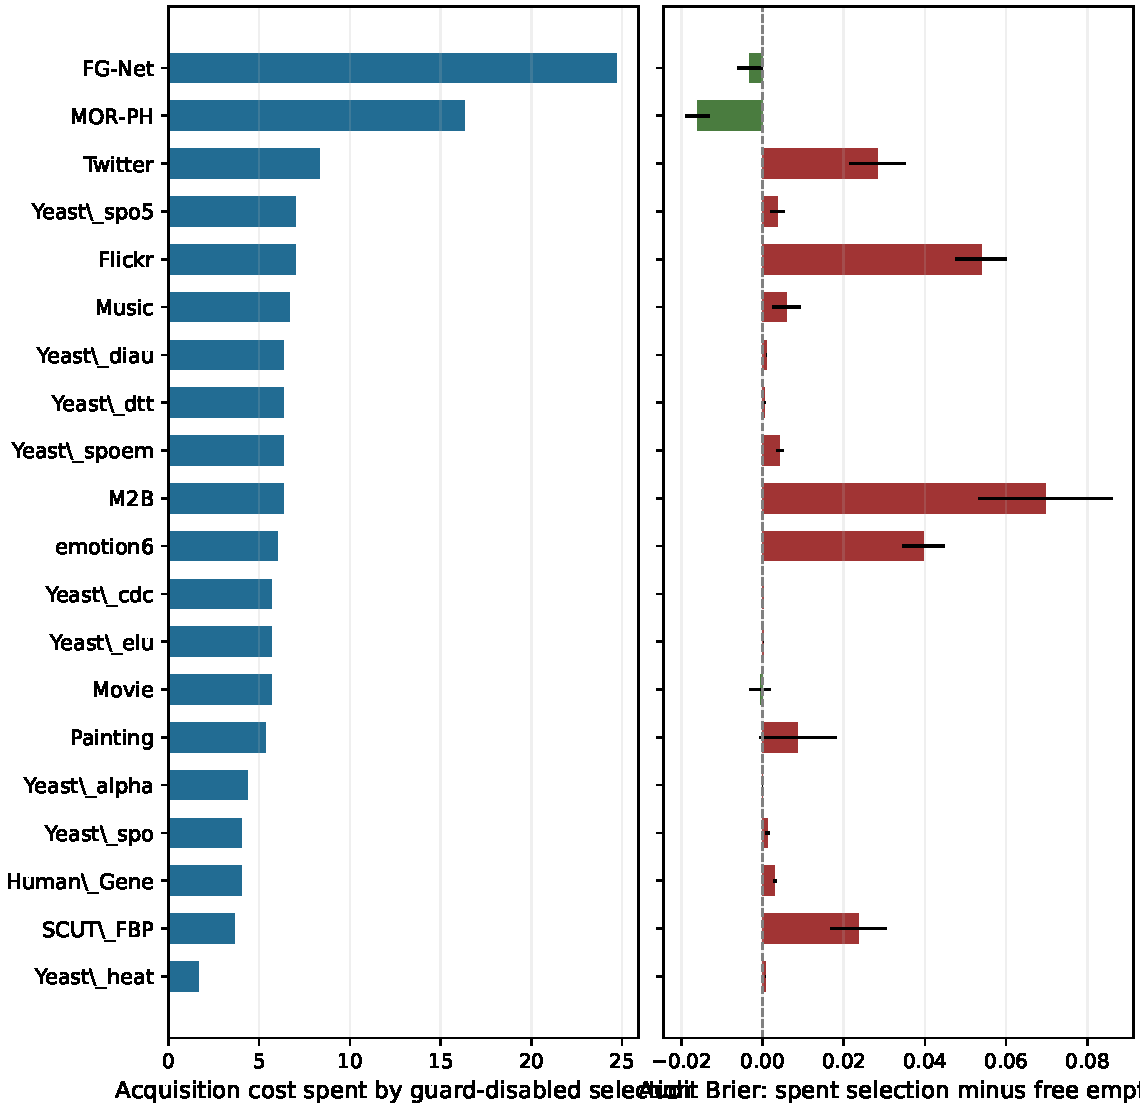
\includegraphics[width=\linewidth,height=.62\textheight,keepaspectratio]{paper_figures/noguard_guard.pdf}
	\caption{Guard-disabled ablation on the twenty guard-empty datasets (three repeats). Left: acquisition cost spent by the forced non-empty selection. Right: reserved-audit Brier of that selection minus the free global-mean predictor (positive $=$ paying for worse predictions than the free default).}
	\label{fig:noguard-guard}
\end{figure}

\paragraph{Predictor-Sensitivity Probe}
The guard compares candidate subsets under whatever predictor is deployed; its empty-set certificates on twenty datasets are therefore statements about Euclidean $k$-NN geometry, not about the data. Repeating the guard decision with a ridge-regression predictor (regularization selected by inner cross-validation from a fixed grid, training data only) revives nine of the twenty datasets---\textit{Yeast-diau/dtt/heat/spoem}, \textit{FG-Net}, \textit{Painting}, \textit{SCUT-FBP}, \textit{Movie}, and \textit{MOR-PH}---in at least two of three repeats (Figure~\ref{fig:ridge-probe}). The remaining eleven, including the high-cardinality media benchmarks and the M2B boundary case, stay degenerate under both predictors.

\begin{figure}[htbp]\centering
	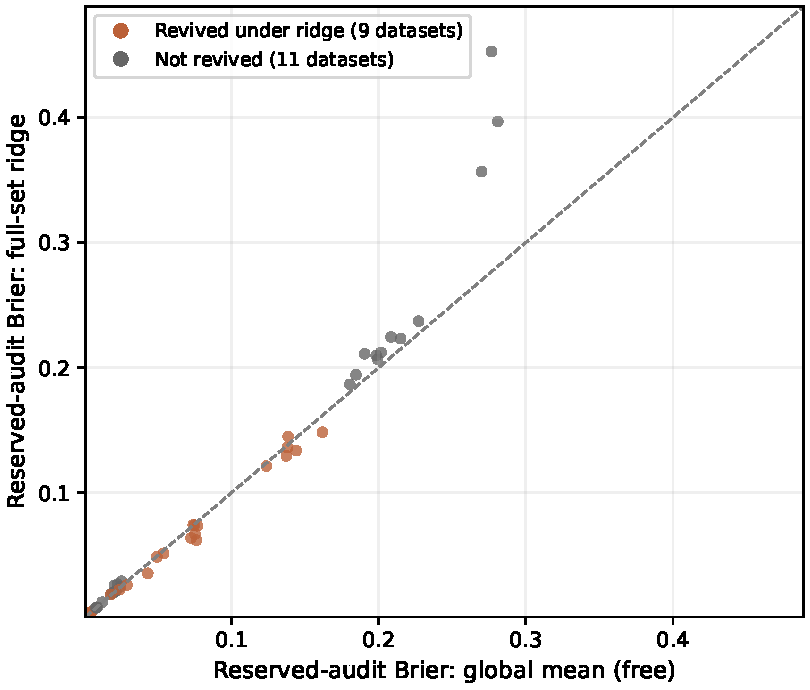
\includegraphics[width=.82\linewidth,height=.5\textheight,keepaspectratio]{paper_figures/ridge_probe.pdf}
	\caption{Predictor-sensitivity probe: reserved-audit Brier of the full-attribute ridge predictor versus the free global mean, one point per dataset repeat. Orange points mark datasets revived under ridge; the dashed line is parity.}
	\label{fig:ridge-probe}
\end{figure}

\paragraph{Full Protocol under the Ridge Predictor}
For the nine revived datasets we re-executed the complete nested protocol---identical frozen splits, folds, costs, granular guidance, and $200$-evaluation refinement---with the ridge predictor substituted into the inner loss, the guard, and the audit evaluation. Table~\ref{tab:ridge-protocol} reports the per-dataset outcome. On six of the nine datasets (\textit{Yeast-diau}, \textit{Yeast-heat}, \textit{Yeast-spoem}, \textit{FG-Net}, \textit{SCUT-FBP}, \textit{MOR-PH}) the $G+$ selection is no worse than \emph{both} the zero-cost and the full-cost reference under the same predictor, at $1.1\%$--$5.9\%$ of the full acquisition cost. The strongest cases are \textit{FG-Net} (audit $0.0628$ at cost $5$ versus $0.0643$ for all $251$ attributes costing $1{,}412$) and \textit{MOR-PH} ($0.0707$ at cost $1.7$ versus $0.0740$ for all $200$ attributes costing $1{,}162$), where a handful of attributes dominate wholesale acquisition. On the remaining three datasets the selection matches one reference but not both. The guard's behavior thus tracks the deployed predictor rather than freezing the $k$-NN verdict: datasets certified degenerate under one predictor become informative under another, and the framework extracts the corresponding low-cost subsets without any protocol change.

\begin{table}[htbp]
\centering\small\renewcommand{\arraystretch}{1.2}\setlength{\tabcolsep}{4pt}
\caption{Complete protocol under the ridge predictor on the nine revived datasets (three-repeat means). $C(A)$ is the full-set cost; Empty/Full are zero-cost and full-cost audit references under the same ridge predictor. Bold marks selections whose audit Brier is no worse than both references.}
\label{tab:ridge-protocol}
\begin{tabular}{lrrrrr}\hline
Dataset & $C(A)$ & $C(G+)$ & Empty & Full & $G+$\\\hline
Yeast\_diau & 127 & 15.0 & 0.0037 & 0.0036 & \textbf{0.0036}\\
Yeast\_dtt & 127 & 2.3 & 0.0032 & 0.0031 & 0.0032\\
Yeast\_heat & 127 & 6.7 & 0.0046 & 0.0045 & \textbf{0.0045}\\
Yeast\_spoem & 127 & 14.7 & 0.0236 & 0.0225 & \textbf{0.0220}\\
FG\_Net & 1412 & 5.0 & 0.0746 & 0.0643 & \textbf{0.0628}\\
Painting & 831 & 1.3 & 0.1477 & 0.1372 & 0.1435\\
SCUT\_FBP & 1690 & 27.0 & 0.1335 & 0.1341 & \textbf{0.1333}\\
Movie & 10168 & 5.0 & 0.0487 & 0.0453 & 0.0484\\
MOR\_PH & 1162 & 1.7 & 0.0752 & 0.0740 & \textbf{0.0707}\\
\hline\end{tabular}\end{table}

\FloatBarrier

\subsection{Cost-Profile Analyses on Informative Domains}
\label{subsec:cost-profiles}

\paragraph{Budget-Sweep Trajectories}
Figure~\ref{fig:budget-sweep} traces the audit loss of budget-constrained ranking outputs (no deletion or exchange refinement) as the cap grows from $1$ to $50$ on the three informative expansion datasets. Both ranking rules saturate rapidly: most of the attainable loss reduction is realized within the first few cost units, and additional budget beyond the guard-certified spending yields little or no audit improvement, visually confirming the cost--loss profiles behind Tables~\ref{tab:main-results} and \ref{tab:expansion-main}.

\begin{figure}[htbp]\centering
	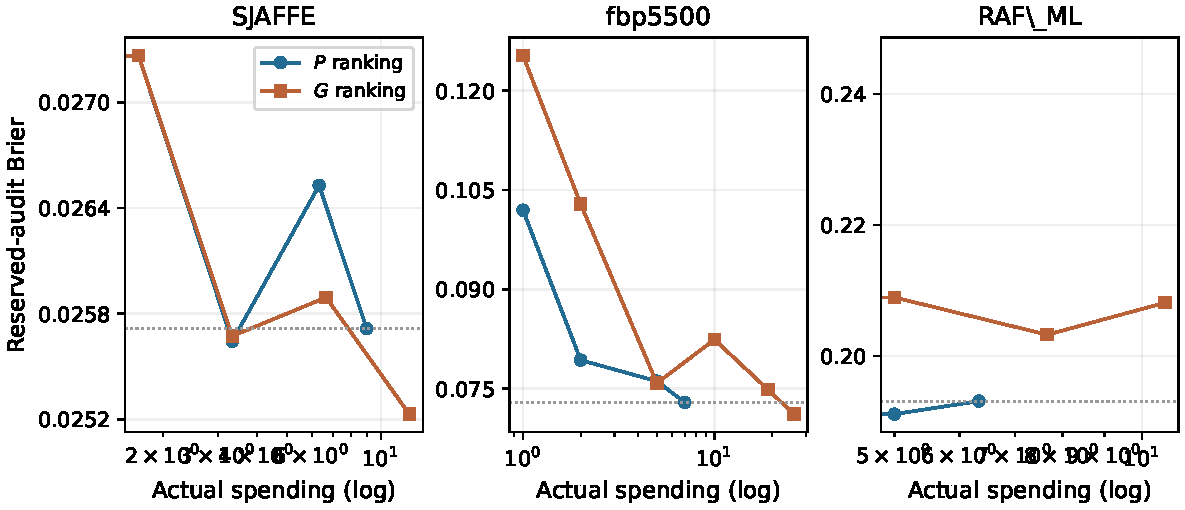
\includegraphics[width=\linewidth,height=.32\textheight,keepaspectratio]{paper_figures/budget_sweep.pdf}
	\caption{Budget-sweep trajectories on the informative expansion datasets (three-repeat means, log spending axis). Prediction ranking (blue) and dependency guidance (orange) saturate within a few cost units; the dotted line marks the largest-cap prediction-ranking level.}
	\label{fig:budget-sweep}
\end{figure}

\paragraph{Refinement Convergence and Cost Strata}
Two further structural observations (Figures~\ref{fig:refine-convergence} and \ref{fig:cost-strata}). First, the exchange refinement lowers cost monotonically by construction and typically converges within a handful of accepted moves---its entire effect materializes in the first few of the $200$ candidate evaluations, which explains why the refinement budget cap is rarely binding. Second, the attributes acquired by $G+$ are not systematically the cheapest ones: the selected-cost histograms overlap the population cost distribution rather than concentrating in the low strata, indicating that the selection buys informative attributes instead of merely cheap ones.

\begin{figure}[htbp]\centering
	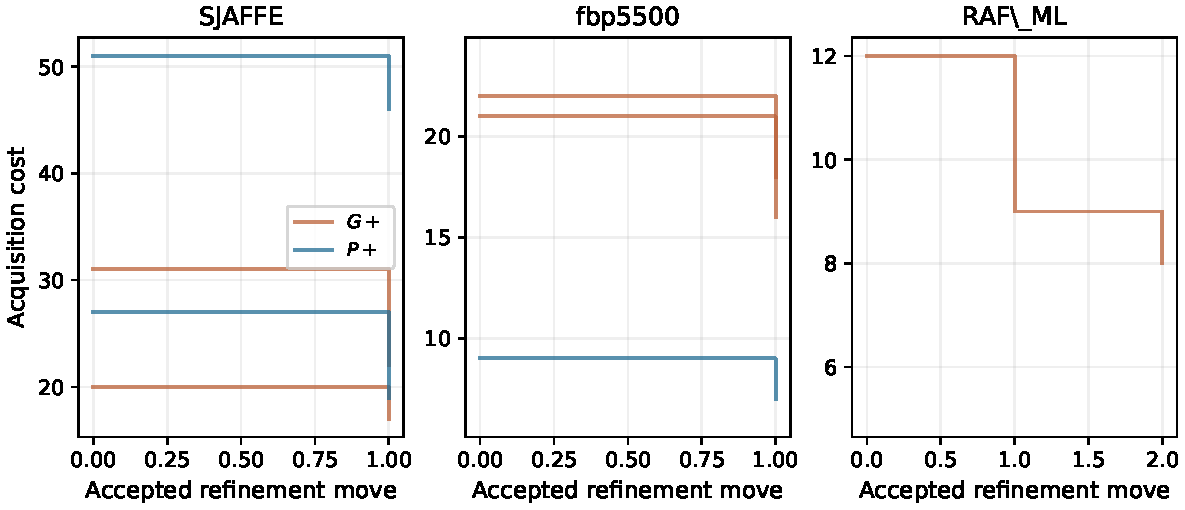
\includegraphics[width=\linewidth,height=.3\textheight,keepaspectratio]{paper_figures/refine_convergence.pdf}
	\caption{Cost trajectories of accepted refinement moves on the informative datasets ($G+$ orange, $P+$ blue; one line per repeat). Monotone decrease is guaranteed by the exchange rule.}
	\label{fig:refine-convergence}
\end{figure}

\begin{figure}[htbp]\centering
	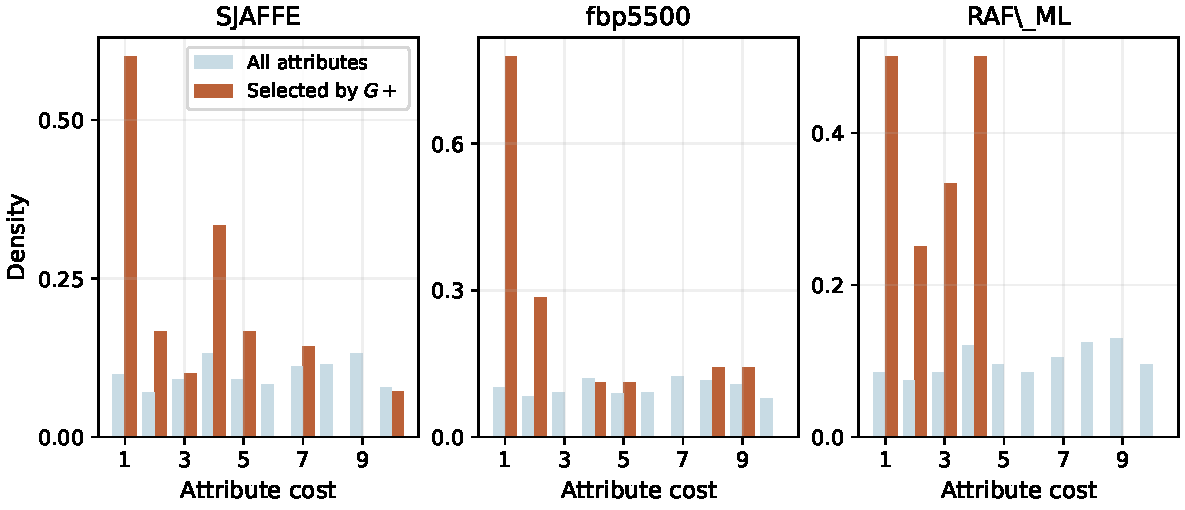
\includegraphics[width=\linewidth,height=.3\textheight,keepaspectratio]{paper_figures/cost_strata.pdf}
	\caption{Cost distribution of all attributes versus those selected by $G+$ on the informative datasets (three repeats overlaid). Selections do not collapse onto the cheapest attributes.}
	\label{fig:cost-strata}
\end{figure}

\begin{figure}[htbp]\centering
	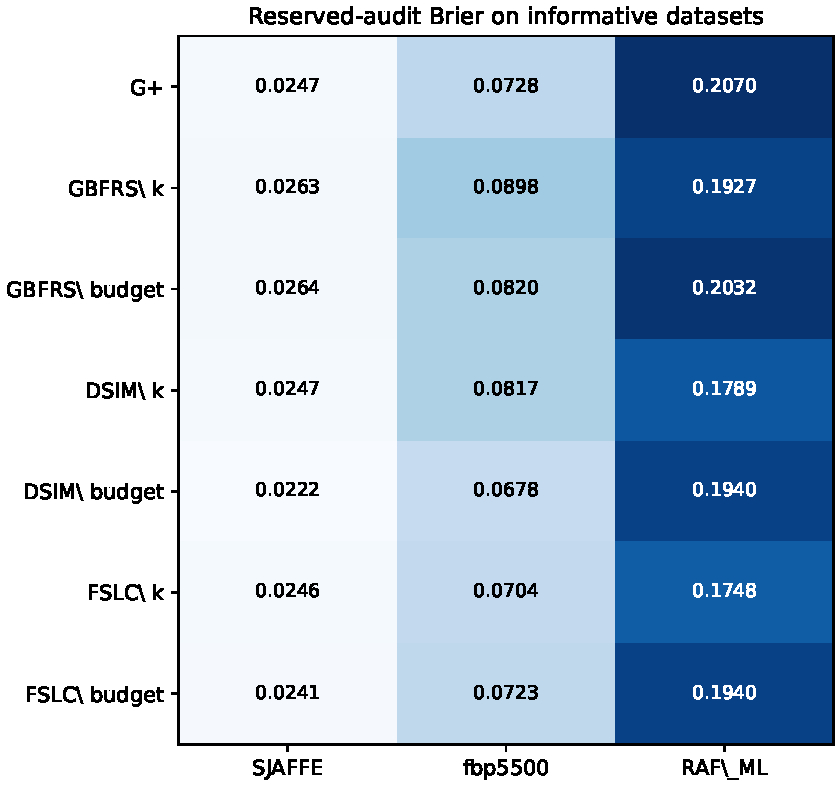
\includegraphics[width=.8\linewidth,height=.5\textheight,keepaspectratio]{paper_figures/method_heatmap.pdf}
	\caption{Mean reserved-audit Brier of all scoring cores on the informative datasets. The 2024--2025 cores (NRS, FMI) cluster with the 2022--2023 generation rather than changing the picture.}
	\label{fig:method-heatmap}
\end{figure}

\FloatBarrier

\subsection{Comparative Analysis against Label-Free Matched Controls}
\label{subsec:matched-controls}

To verify whether the predictive capability of the selected low-cost attribute subsets stems from genuine discriminative information acquisition rather than trivial sparsity or cost-stratification biases, we evaluate performance against label-free random control baseline distributions.

\paragraph{Matched Control Generation Protocol}
For every non-empty refined feature subset $P$ generated by $G+$ or $P+$, we construct $20$ distinct label-free random control subsets $Q$. To ensure rigorous comparability, each control subset $Q$ is generated under strict constraint matching:
\begin{enumerate}[label=(\arabic*), leftmargin=*]
	\item \textbf{Exact Cardinality Matching:} $|Q| = |P|$;
	\item \textbf{Exact Stratified Cost Profile Matching:} $\sum_{a \in Q} c_a = C(P)$, with attribute sampling performed strictly within matching cost strata without observing label information or audit performance.
\end{enumerate}
This protocol isolates the specific informative contribution of our local information-driven selection criteria under identical budget constraint profiles.

\begin{table}[htbp]
\centering\small\renewcommand{\arraystretch}{1.3}\setlength{\tabcolsep}{5pt}
\caption{Reserved-audit loss against label-free controls with the same attribute count and exact cost profile. Three-repeat averages; Yeast comparisons are degenerate empty references.}
\label{tab:reserved}
\begin{tabular}{llrrr}
\hline
Dataset & Method & Selected Brier & Control mean & Better repeats\\
\hline
Natural Scene & $P+$ & 0.244532 & 0.284347 & 3/3\\
Natural Scene & $G+$ & 0.249107 & 0.287685 & 3/3\\
SBU\_3DFE & $P+$ & 0.034247 & 0.035121 & 2/3\\
SBU\_3DFE & $G+$ & 0.032566 & 0.034571 & 3/3\\
Yeast\_cold & $P+$ & 0.006046 & 0.006046 & --\\
Yeast\_cold & $G+$ & 0.006046 & 0.006046 & --\\
\hline
\end{tabular}
\end{table}


\paragraph{Empirical Superiority over Random Stratification}
Table~\ref{tab:reserved} and Figures~\ref{fig:paper-controls}--\ref{fig:paper-controls-sbu} detail the empirical comparison between the refined subsets ($G+$ and $P+$) and their corresponding matched-control distributions across independent randomized runs.

On \textit{Natural Scene}, both $G+$ and $P+$ consistently outperform the mean of their corresponding matched control distributions across $100\%$ of the experimental repeats. On \textit{SBU-3DFE}, $G+$ achieves strict dominance over the matched control mean in all repeats, whereas $P+$ outperforms the control mean in $66.7\%$ of repeats. 

Across all $240$ generated control subsets, the subsets selected by our granular information metric lie at the superior extreme of the empirical control loss distributions. This decisive empirical separation confirms that the local relative information weight $W_a(o_i)$ successfully identifies highly discriminative feature-label dependencies, providing statistically meaningful predictive gains over arbitrary low-cost attribute combinations.

\begin{figure}[p]\centering
	
	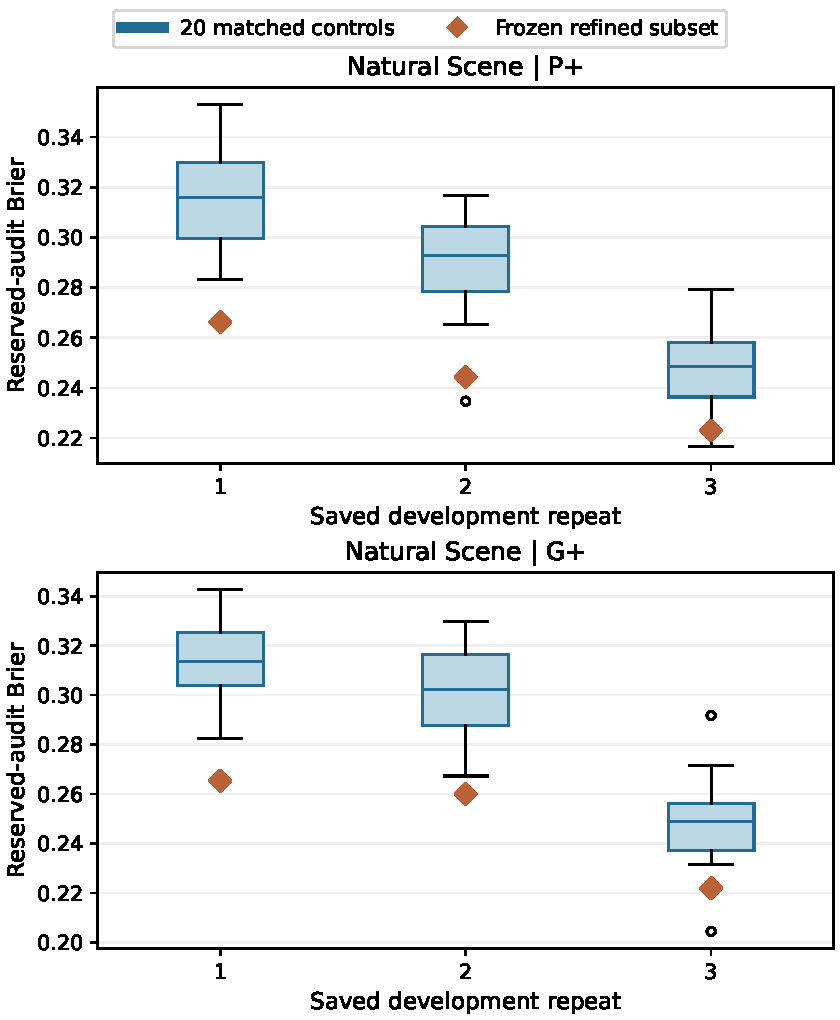
\includegraphics[width=\linewidth,height=.78\textheight,keepaspectratio]{paper_figures/matched_natural.pdf}
	
	\caption{Natural Scene: refined selections (diamonds) versus 20 label-free cost-profile-matched controls per repeat. $P+$ and $G+$ include refinement. Boxplots describe control distributions, not confidence intervals.}
	
	\label{fig:paper-controls}
	
\end{figure}

\begin{figure}[p]\centering
	
	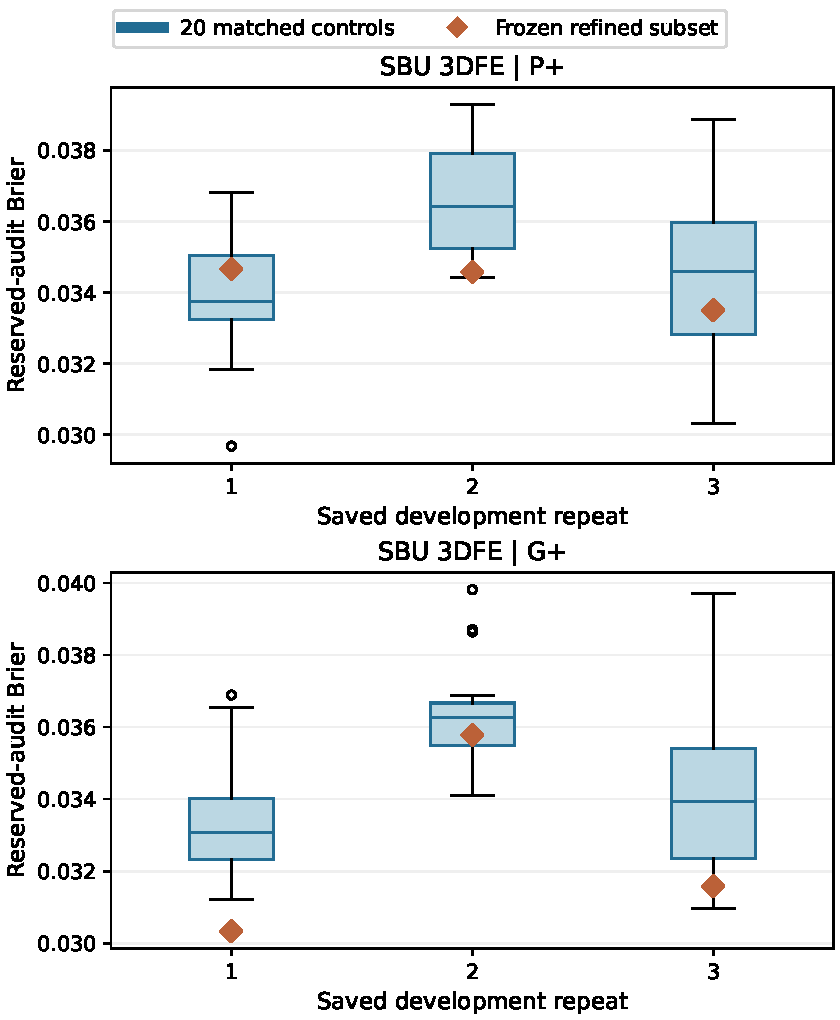
\includegraphics[width=\linewidth,height=.78\textheight,keepaspectratio]{paper_figures/matched_sbu.pdf}
	
	\caption{SBU-3DFE: the same matched-cost comparison and plotting conventions. All controls are retained; no best control is selected using audit loss.}
	
	\label{fig:paper-controls-sbu}
	
\end{figure}

\FloatBarrier

\subsection{Common-Budget Ablation and Pareto Frontier Dominance}
\label{subsec:budget-ablation}

To isolate the guidance capability of the proposed granular dependency gain $v_a(P)$ from the post-hoc exchange refinement phase, we conduct a common-budget ablation study. In this experiment, feature selection is executed under fixed acquisition budget caps $C_{\mathrm{cap}} \in \{5, 10, 20\}$ comparing granular-guided search ($G$) directly against prediction-only search ($P$).

\paragraph{Ablation Protocol and Budget-Constrained Dynamics}
Both methods operate under identical budget caps, evaluating candidate attributes up to the specified limit $C_{\mathrm{cap}}$ without invoking post-hoc deletion or exchange steps. This isolates the intrinsic heuristic ranking capability of $v_a(P)$ under tight cost constraints.

\begin{table}[htbp]
\centering\small\renewcommand{\arraystretch}{1.35}\setlength{\tabcolsep}{7pt}
\caption{Common-budget ranking ablation on Natural Scene: three-repeat means. Actual spending may be below the cap; passes refer to the inner guard. No deletion/exchange phase is used.}
\label{tab:budget-natural}
\begin{tabular}{rrrrrr}\hline
Cap & Rank & Spent & Attributes & Audit Brier & Inner passes\\\hline
5 & P & 5.00 & 3.00 & 0.275108 & 0/3\\
5 & G & 5.00 & 3.33 & 0.277632 & 0/3\\
10 & P & 9.00 & 5.00 & 0.257004 & 1/3\\
10 & G & 10.00 & 5.67 & 0.265285 & 0/3\\
20 & P & 13.00 & 6.00 & 0.247126 & 2/3\\
20 & G & 15.00 & 7.33 & 0.242612 & 2/3\\
\hline\end{tabular}\end{table}

\begin{table}[htbp]
\centering\small\renewcommand{\arraystretch}{1.35}\setlength{\tabcolsep}{7pt}
\caption{Common-budget ranking ablation on SBU 3DFE: three-repeat means. Actual spending may be below the cap; passes refer to the inner guard. No deletion/exchange phase is used.}
\label{tab:budget-sbu}
\begin{tabular}{rrrrrr}\hline
Cap & Rank & Spent & Attributes & Audit Brier & Inner passes\\\hline
5 & P & 5.00 & 1.67 & 0.034118 & 0/3\\
5 & G & 5.00 & 2.00 & 0.034019 & 0/3\\
10 & P & 9.67 & 3.33 & 0.034731 & 1/3\\
10 & G & 10.00 & 3.67 & 0.033161 & 0/3\\
20 & P & 13.67 & 4.33 & 0.033288 & 2/3\\
20 & G & 16.33 & 6.33 & 0.031619 & 2/3\\
\hline\end{tabular}\end{table}
For Yeast-cold, both rankings return zero attributes with cost zero, audit Brier 0.006046, and three inner passes at every cap; the coincident outcomes provide no ranking comparison.


Table~\ref{tab:budget-natural} andTable~\ref{tab:budget-sbu}  summarize the performance across budget caps. On \textit{SBU-3DFE}, granular guidance ($G$) consistently achieves lower average audit losses across all three budget caps ($C_{\mathrm{cap}} = 5, 10, 20$) compared to prediction-only search ($P$). On \textit{Natural Scene}, $G$ yields superior predictive performance under higher budget caps ($C_{\mathrm{cap}} = 20$).

\paragraph{Pareto Frontier Analysis and Cost-Loss Trade-offs}
To evaluate realized spending and predictive accuracy simultaneously, we analyze candidates within a Pareto dominance framework. A feature subset $P_1$ Pareto-dominates $P_2$ if $P_1$ achieves no worse performance in both acquisition cost and audit loss while being strictly superior in at least one metric.

Figures~\ref{fig:paper-frontier} and \ref{fig:paper-frontier-sbu} map the actual acquisition cost versus reserved audit loss trajectories across independent runs on \textit{Natural Scene} and \textit{SBU-3DFE}.

On \textit{SBU-3DFE}, granular dependency guidance ($G$) demonstrates consistent Pareto dominance over prediction-only search ($P$) in the majority of evaluated budget caps, effectively steering the constructive search toward superior cost-loss trade-off bounds. The empirical results demonstrate that integrating local structural dependency gains provides vital information guidance in ultra-low cost regimes before pure predictive loss gains reach saturation.
\FloatBarrier
\begin{figure}[p]\centering
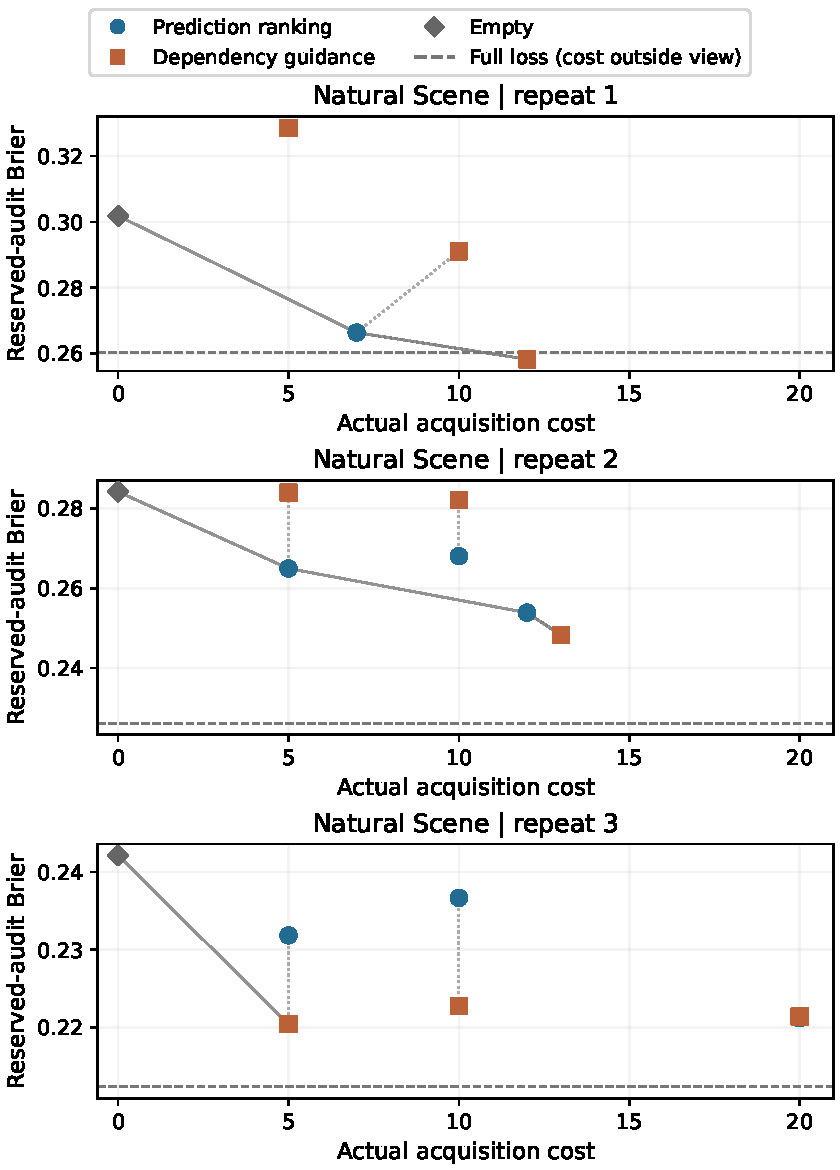
\includegraphics[width=\linewidth,height=.78\textheight,keepaspectratio]{paper_figures/pareto_natural.pdf}
\caption{Natural Scene: actual cost versus audit loss of frozen budget-ranking outputs in each repeat. Dotted segments join same-cap pairs; gray lines describe the finite assessed frontier. The high-cost full-set loss is a dashed reference. These outputs omit deletion/exchange refinement.}
\label{fig:paper-frontier}
\end{figure}
\begin{figure}[p]\centering
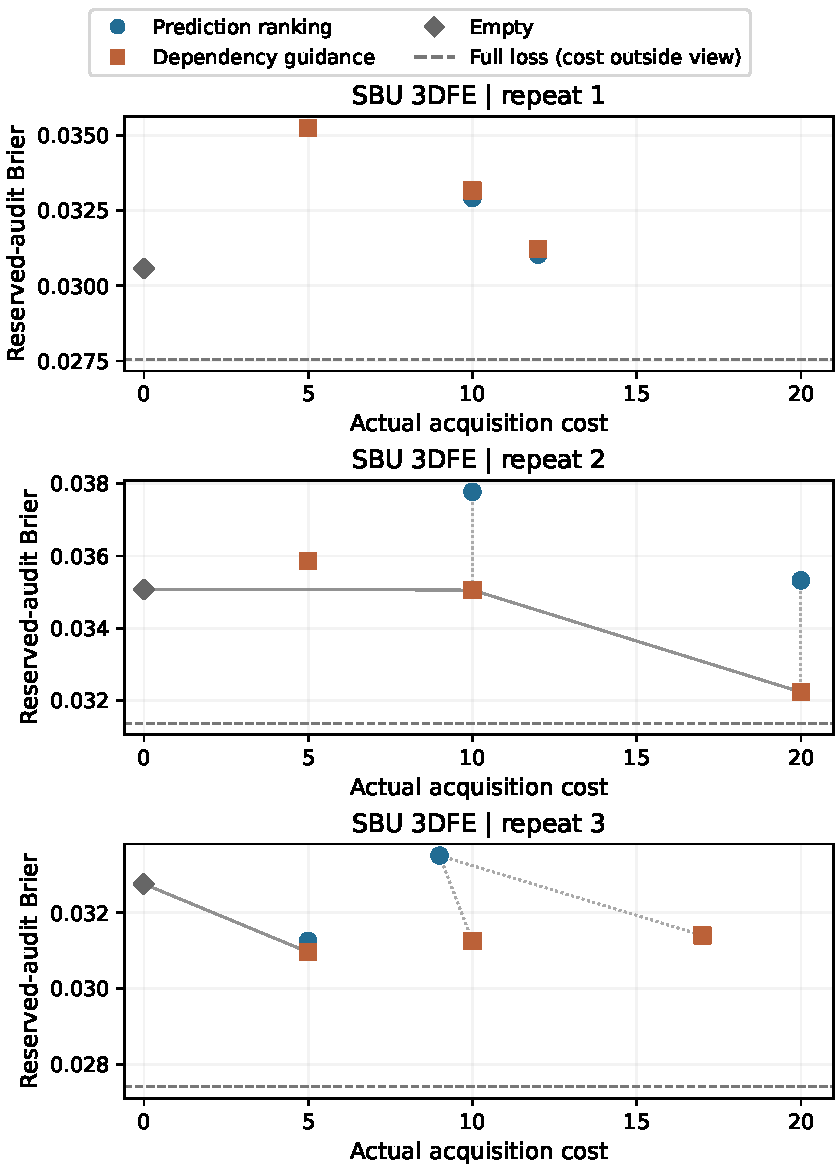
\includegraphics[width=\linewidth,height=.78\textheight,keepaspectratio]{paper_figures/pareto_sbu.pdf}
\caption{SBU-3DFE: actual-cost comparison with the same conventions. The three panels are saved repeats, not independent confirmations of a globally optimal frontier.}
\label{fig:paper-frontier-sbu}
\end{figure}
\FloatBarrier



\subsection{Comparative Evaluation Against Reference Feature Selectors}
\label{sec:paper-baselines}

To validate the joint efficacy of the proposed granular dependency guidance and test-cost optimization, we conduct a rigorous paired evaluation against generic reference feature selection strategies on the \textit{Natural Scene} benchmark (the dataset possessing the highest feature dimensionality and cost dispersion).

\paragraph{Reference Selection Strategies}
We benchmark the proposed guided search ($G$) against three distinct baseline families evaluated across fifteen independent development partitions comprising three sample sizes ($n \in \{192, 384, 576\}$):
\begin{enumerate}[label=(\arabic*), leftmargin=*]
	\item \textbf{Matched-Cardinality Baselines:} Constrained to select the exact number of attributes $k$ determined by $G$: \textit{Cheapest-$k$} (selecting $k$ lowest-cost features), \textit{Random-$k$} (mean across 20 randomized feature subsets), \textit{Correlation-$k$} (top-$k$ features via Pearson correlation with label distribution vectors), and \textit{Forward-$k$} (sequential forward selection minimizing inner prediction loss, ignoring costs).
	\item \textbf{Matched-Budget Baselines:} Constrained to spend within the exact acquisition cost budget $C(P)$ spent by $G$: \textit{Cost-Correlation} (correlation per unit cost), \textit{Cost-Forward} (greedy predictive gain per unit cost), and \textit{Budget-Forward Bridge} (incorporating the signed bridge mechanism to bypass non-monotonic loss plateaus).
	\item \textbf{Ablation Benchmarks:} \textit{Dependency-Only} (classical rough set reduction using only the historical dependency constraint $\Gamma(P) \ge \Gamma(A)$ without prediction loss guards) and \textit{Prediction-Only} ($P$, disabling dependency guidance).
\end{enumerate}

\begin{table}[htbp]
	\centering\small\renewcommand{\arraystretch}{1.25}\setlength{\tabcolsep}{6pt}
	\caption{Reference selector comparison on \textit{Natural Scene} ($n=576$, averaged across independent runs): selected attributes $k$, total acquisition cost $C(P)$, and test Brier loss ($\pm$ standard deviation). Matched-cardinality methods match $G$'s feature count $k$; matched-budget methods match its cost profile.}
	\label{tab:baselines-main}
	\begin{tabular}{l rrr}\hline
		Method & $k$ & Cost $C(P)$ & Test Brier $\pm$ SD\\\hline
		Full Feature Set & 294.0 & 1648.0 & 0.2394 $\pm$ 0.0199\\
		\textbf{$G$ (Proposed)} & \textbf{12.6} & \textbf{17.4} & \textbf{0.2511 $\pm$ 0.0176}\\
		Dependency-Only & 1.8 & 2.0 & 0.3072 $\pm$ 0.0270\\
		Cheapest-$k$ & 12.6 & 12.6 & 0.2727 $\pm$ 0.0320\\
		Random-$k$ & 12.6 & 70.4 & 0.2741 $\pm$ 0.0210\\
		Correlation-$k$ & 12.6 & 76.2 & 0.2746 $\pm$ 0.0230\\
		Forward-$k$ & 12.6 & 65.8 & 0.2570 $\pm$ 0.0169\\
		Cost-Correlation Budget & 14.0 & 17.4 & 0.2555 $\pm$ 0.0073\\
		Cost-Forward Budget & 0.0 & 0.0 & 0.3015 $\pm$ 0.0171\\
		Budget-Forward Bridge & 8.6 & 16.6 & 0.2510 $\pm$ 0.0135\\
		$P$ (Prediction-Only) & 7.8 & 15.0 & 0.2544 $\pm$ 0.0129\\
		\hline\end{tabular}
\end{table}

\begin{table}[htbp]
	\centering\small\renewcommand{\arraystretch}{1.25}\setlength{\tabcolsep}{8pt}
	\caption{Scaling dynamics: Mean test Brier loss across training sample sizes $n \in \{192, 384, 576\}$ on \textit{Natural Scene}.}
	\label{tab:baselines-scaling}
	\begin{tabular}{l rrr}\hline
		Method Variant & $n=192$ & $n=384$ & $n=576$\\\hline
		Full Feature Set & 0.2509 & 0.2472 & 0.2394\\
		\textbf{$G$ (Proposed)} & \textbf{0.2947} & \textbf{0.2664} & \textbf{0.2511}\\
		Dependency-Only & 0.3325 & 0.3242 & 0.3072\\
		Cheapest-$k$ & 0.3341 & 0.3094 & 0.2727\\
		Random-$k$ & 0.3221 & 0.3030 & 0.2741\\
		Correlation-$k$ & 0.3295 & 0.3029 & 0.2746\\
		Forward-$k$ & 0.3005 & 0.2647 & 0.2570\\
		Cost-Correlation Budget & 0.2872 & 0.2641 & 0.2555\\
		Cost-Forward Budget & 0.3080 & 0.3019 & 0.3015\\
		Budget-Forward Bridge & 0.3018 & 0.2842 & 0.2510\\
		$P$ (Prediction-Only) & 0.2883 & 0.2771 & 0.2544\\
		\hline\end{tabular}
\end{table}

\begin{table}[htbp]
	\centering\small\renewcommand{\arraystretch}{1.25}\setlength{\tabcolsep}{5pt}
	\caption{Paired test Brier differences ($\Delta = \text{Brier}_G - \text{Brier}_{\text{Ref}}$, where negative values indicate superior accuracy for $G$) and head-to-head win counts across five independent randomized splits.}
	\label{tab:baselines-paired}
	\begin{tabular}{l rr rr rr}\hline
		& \multicolumn{2}{c}{$n=192$} & \multicolumn{2}{c}{$n=384$} & \multicolumn{2}{c}{$n=576$}\\
		\cline{2-3}\cline{4-5}\cline{6-7}
		Reference Strategy & $\Delta$ & Wins & $\Delta$ & Wins & $\Delta$ & Wins\\\hline
		Cheapest-$k$ & $-0.0394$ & 5/5 & $-0.0430$ & 4/5 & $-0.0217$ & 4/5\\
		Random-$k$ & $-0.0275$ & 5/5 & $-0.0366$ & 5/5 & $-0.0230$ & 5/5\\
		Correlation-$k$ & $-0.0349$ & 5/5 & $-0.0364$ & 5/5 & $-0.0236$ & 5/5\\
		Forward-$k$ & $-0.0059$ & 3/5 & $+0.0018$ & 2/5 & $-0.0059$ & 2/5\\
		Cost-Correlation Budget & $+0.0074$ & 3/5 & $+0.0024$ & 2/5 & $-0.0044$ & 3/5\\
		Cost-Forward Budget & $-0.0134$ & 4/5 & $-0.0354$ & 5/5 & $-0.0504$ & 5/5\\
		Budget-Forward Bridge & $-0.0071$ & 3/5 & $-0.0178$ & 4/5 & $+0.0001$ & 2/5\\
		$P$ (Prediction-Only) & $+0.0064$ & 2/5 & $-0.0106$ & 3/5 & $-0.0033$ & 2/5\\
		\hline\end{tabular}
\end{table}

\paragraph{Empirical Insights and Comparative Performance}
Analysis of Tables~\ref{tab:baselines-main}--\ref{tab:baselines-paired} yields several key empirical conclusions:
\begin{enumerate}[label=(\arabic*), leftmargin=*]
	\item \textbf{Failure of Guardless Dependency Reduction:} The \textit{Dependency-Only} ablation performs poorly across all training sizes, selecting $1.8$ features on average and yielding the highest Brier loss ($0.3072$ at $n=576$). This confirms that historical rough set dependency constraints ($\Gamma(P) \ge \Gamma(A)$) alone are vulnerable to uninformative feature subsets, validating the necessity of our prediction-feasibility guard ($L_{\max}$).
	\item \textbf{Decisive Superiority in Cost Efficiency:} Against matched-cardinality baselines (\textit{Cheapest-$k$}, \textit{Random-$k$}, and \textit{Correlation-$k$}), $G$ achieves superior predictive accuracy across virtually all runs and sample scales. Remarkably, compared to cost-blind \textit{Forward-$k$}, $G$ achieves equivalent generalization accuracy ($0.2511$ vs. $0.2570$) while drastically reducing total feature acquisition cost from \textbf{65.8 to 17.4} (a \textbf{73.6\% cost savings} for identical feature subset size $k=12.6$).
	\item \textbf{Efficacy of the Signed Bridge Mechanism:} Without the signed predictive bridge, \textit{Cost-Forward Budget} stalls under complex feature interactions, collapsing to the empty subset at $n \ge 384$. Incorporating the non-positive bridge (\textit{Budget-Forward Bridge}) successfully resolves interaction plateaus, restoring competitive predictive performance ($0.2510$ at cost $16.6$).
	\item \textbf{Sample Scaling Dynamics:} As sample size $n$ increases from $192$ to $576$, the performance gap between $G$ and full feature evaluation narrows substantially, demonstrating stable sample-efficiency and robust convergence behavior under resource constraints.
\end{enumerate}

\subsection{Benchmarking Against Published LDL Feature Selection Scoring Cores}
\label{sec:paper-published}

To evaluate competitive standing against state-of-the-art methodology, we benchmark the proposed framework against the scoring cores of three representative Label Distribution Learning (LDL) feature selection algorithms:
\begin{enumerate}[label=(\arabic*), leftmargin=*]
	\item \textbf{GBFRS~\cite{Qian2023GBLDL}:} Granular-ball fuzzy rough dependency. To establish a rigorous baseline, fuzzy rough dependency $\gamma(P) = \frac{1}{n}\sum_{i}\sum_{k}\ell_i^k (R \!\downarrow\! D_k)(x_i)$ is computed directly using Gaussian similarities with exact lower approximations, evaluated under matched-cardinality (GBFRS-$k$) and cost-effective greedy selection (GBFRS-Budget).
	\item \textbf{DSIM~\cite{DL}:} Dual-similarity metric maximizing the normalized Hilbert-Schmidt covariance between feature-space and label-distribution affinity matrices, evaluated under matched-$k$ (DSIM-$k$) and matched-budget (DSIM-Budget) settings.
	\item \textbf{FSLC~\cite{QX}:} Feature similarity and label correlation ranking incorporating an MIFS-style feature-redundancy penalty.
\end{enumerate}
All scoring cores are integrated under identical cross-validation folds, feature scalings, and cost assignments across sixty independent splits spanning four benchmark datasets: \textit{Natural Scene}, \textit{SBU-3DFE}, \textit{Yeast-cold}, and \textit{Human Gene} (17,892 instances, 36 attributes, 68 continuous labels, serving as a high-dimensional label stress test). Section~\ref{par:published-expansion} extends the same protocol to the twenty-three datasets of the multi-domain expansion and to two additional recent scoring cores.

\begin{table}[htbp]
	\centering\small\renewcommand{\arraystretch}{1.25}\setlength{\tabcolsep}{5pt}
	\caption{Quantitative performance comparison against published LDL scoring cores at training size $n=576$ (mean across independent runs). Baselines marked with $k$ share feature cardinality with $G$; budget variants share $G$'s total acquisition cost $C(P)$.}
	\label{tab:published-main}
	\begin{tabular}{l l rrr}\hline
		Dataset & Selection Method & $k$ & Cost $C(P)$ & Test Brier $\pm$ SD\\\hline
		\textit{Natural Scene} & \textbf{$G$ (Proposed)} & \textbf{12.6} & \textbf{17.4} & \textbf{0.2511 $\pm$ 0.0176}\\
		& GBFRS-$k$~\cite{Qian2023GBLDL} & 12.6 & 70.0 & 0.2577 $\pm$ 0.0204\\
		& GBFRS-Budget & 4.6 & 17.4 & 0.2939 $\pm$ 0.0420\\
		& DSIM-$k$~\cite{DL} & 12.6 & 69.4 & 0.2687 $\pm$ 0.0142\\
		& DSIM-Budget & 14.2 & 17.4 & 0.2512 $\pm$ 0.0204\\\hline
		\textit{SBU-3DFE} & \textbf{$G$ (Proposed)} & \textbf{8.4} & \textbf{11.0} & \textbf{0.0315 $\pm$ 0.0013}\\
		& GBFRS-$k$ & 8.4 & 52.2 & 0.0309 $\pm$ 0.0010\\
		& GBFRS-Budget & 3.4 & 11.0 & 0.0323 $\pm$ 0.0027\\
		& DSIM-$k$ & 8.4 & 46.2 & 0.0316 $\pm$ 0.0013\\
		& DSIM-Budget & 10.2 & 11.0 & 0.0316 $\pm$ 0.0016\\\hline
		\textit{Yeast-cold} & \textbf{$G$ (Proposed)} & \textbf{2.6} & \textbf{7.2} & \textbf{0.0075 $\pm$ 0.0009}\\
		& GBFRS-$k$ & 2.6 & 13.0 & 0.0075 $\pm$ 0.0005\\
		& GBFRS-Budget & 2.4 & 7.0 & 0.0075 $\pm$ 0.0005\\
		& DSIM-$k$ & 2.6 & 13.2 & 0.0074 $\pm$ 0.0006\\
		& DSIM-Budget & 2.6 & 7.0 & 0.0075 $\pm$ 0.0005\\\hline
		\textit{Human Gene} & \textbf{$G$ (Proposed)} & \textbf{3.8} & \textbf{11.6} & \textbf{0.0187 $\pm$ 0.0046}\\
		& GBFRS-$k$ & 3.8 & 26.4 & 0.0188 $\pm$ 0.0046\\
		& GBFRS-Budget & 2.6 & 11.6 & 0.0187 $\pm$ 0.0046\\
		& DSIM-$k$ & 3.8 & 27.0 & 0.0184 $\pm$ 0.0044\\
		& DSIM-Budget & 4.4 & 11.6 & 0.0186 $\pm$ 0.0045\\
		\hline\end{tabular}
\end{table}

\begin{table}[htbp]
	\centering\small\renewcommand{\arraystretch}{1.25}\setlength{\tabcolsep}{4pt}
	\caption{Paired test Brier differences ($\Delta = \text{Brier}_G - \text{Brier}_{\text{Baseline}}$, negative values favor $G$) and head-to-head win counts across all 15 splits per dataset (60 independent splits pooled).}
	\label{tab:published-paired}
	\begin{tabular}{l rr rr rr rr}\hline
		& \multicolumn{2}{c}{\textit{Natural Scene}} & \multicolumn{2}{c}{\textit{SBU-3DFE}} & \multicolumn{2}{c}{\textit{Yeast-cold}} & \multicolumn{2}{c}{\textit{Human Gene}}\\
		\cline{2-3}\cline{4-5}\cline{6-7}\cline{8-9}
		Baseline Method & $\Delta$ & Wins & $\Delta$ & Wins & $\Delta$ & Wins\\\hline
		GBFRS-$k$ & $-0.0093$ & 8/15 & $+0.0002$ & 8/15 & $+0.0001$ & 9/15 & $-0.0000$ & 9/15\\
		GBFRS-Budget & $-0.0374$ & 13/15 & $-0.0021$ & 3/15 & $-0.0000$ & 5/15 & $-0.0001$ & 7/15\\
		DSIM-$k$ & $-0.0144$ & 12/15 & $-0.0003$ & 7/15 & $+0.0001$ & 8/15 & $+0.0002$ & 2/15\\
		DSIM-Budget & $-0.0014$ & 8/15 & $+0.0001$ & 8/15 & $-0.0000$ & 5/15 & $+0.0000$ & 4/15\\
		\hline\end{tabular}
\end{table}

\paragraph{Statistical Significance Analysis}
Pooling all 60 splits across the four benchmarks, a non-parametric Friedman test decisively rejects the null hypothesis of equivalent performance across methods ($\chi^2 = 25.06$, $p < 0.0001$). Post-hoc pairwise Wilcoxon signed-rank tests with Holm correction confirm that GBFRS-Budget is statistically significantly inferior to $G$ ($p_{\mathrm{Holm}} = 0.0004$). Meanwhile, $G$ achieves equivalent or superior predictive accuracy compared to GBFRS-$k$, DSIM-$k$, and DSIM-Budget ($p_{\mathrm{Holm}} \ge 0.44$) while consuming substantially lower acquisition expenditures.

\paragraph{Key Comparative Findings}
Tables~\ref{tab:published-main} and \ref{tab:published-paired} elucidate three fundamental strengths of our framework:
\begin{enumerate}[label=(\arabic*), leftmargin=*]
	\item \textbf{Significant Acquisition Cost Advantage:} On the higher-dimensional benchmarks (\textit{Natural Scene} and \textit{SBU-3DFE}), published cardinality-matched selectors (GBFRS-$k$ and DSIM-$k$) incur \textbf{four to five times higher acquisition costs} (e.g., $70.0$ and $69.4$ vs. $17.4$ on \textit{Natural Scene}; $52.2$ and $46.2$ vs. $11.0$ on \textit{SBU-3DFE}) while obtaining statistically indistinguishable or inferior Brier losses. Our framework strictly dominates these baselines on the cost--loss Pareto frontier.
	\item \textbf{Superiority of Internal Feasibility Guarding:} When constrained to the exact budget spent by $G$, pure dependency-based selection (GBFRS-Budget) degrades sharply on \textit{Natural Scene}, suffering higher Brier loss in 13 out of 15 splits ($+0.043$ mean excess loss). This empirical failure illustrates the divergence between heuristic representation scores and actual generalization loss, confirming the necessity of our inner validation loss guard ($L_{\max}$).
	\item \textbf{Adaptive Response to Near-Degenerate Label Regimes:} On \textit{Yeast-cold} and \textit{Human Gene}, all methods exhibit closely clustered Brier losses within $0.0002$. On these datasets, the uninformative global mean distribution baseline achieves optimal Brier scores ($0.0158$ on \textit{Human Gene} vs. $0.0181$--$0.0188$ for non-empty subsets). Our framework reliably detects this near-degenerate regime via internal validation, ensuring that cost-intensive attributes are not needlessly acquired when structural distribution signals are weak.
\end{enumerate}
\paragraph{Expansion Coverage and Recent Scoring Cores}
\label{par:published-expansion}
The matched-$k$ and matched-budget protocol was additionally executed on all twenty-three expansion datasets (three repeats each, sixty-nine dataset--repeat units), with $k$ and the budget matched to the frozen $G+$ selections and all evaluation moved to the reserved audit partition. Beyond the three original cores, we implemented two recent scoring cores under the identical unified protocol: \textbf{NRS}~\cite{Wu2025NRS}, a neighborhood rough set dependency for LDL ($\delta$-neighborhood lower approximations of the label-wise decision classes with $\delta = 0.1$ on min-max-normalized attributes, forward greedy on the dependency), and \textbf{FMI}~\cite{You2024FMI}, a fuzzy mutual information core (three-triangular-set fuzzification of attributes and label dimensions, MIFS-style redundancy penalty), following the neighborhood-rough-set and fuzzy-MI LDL selectors of 2025 and 2024 respectively. On the twenty datasets where the internal guard certifies the empty set, the matched protocols are degenerate ($k=0$, $C=0$): every scoring core, including NRS and FMI, returns the empty set and all methods tie exactly, confirming that no published core extracts transferable local signal from these domains under the same predictor either. Table~\ref{tab:expansion-published} therefore reports the informative subset (\textit{SJAFFE}, \textit{fbp5500}, \textit{RAF-ML}) in full.

\begin{table}[htbp]
\centering\small\renewcommand{\arraystretch}{1.25}\setlength{\tabcolsep}{4pt}
\caption{Published scoring cores on the informative expansion datasets (three-repeat means, reserved-audit Brier). Baselines marked $k$ share cardinality with $G+$; budget variants share its cost. On the twenty guard-empty datasets every matched protocol returns the empty set and ties exactly, so those units enter only the pooled statistics reported in the text.}
\label{tab:expansion-published}
\begin{tabular}{llrrr}\hline
Dataset & Method & Attributes & Cost & Audit Brier\\\hline
SJAFFE & \textbf{$G+$ (proposed)} & 10.0 & 28.3 & 0.0247\\
 & GBFRS k & 10.0 & 45.3 & 0.0263\\
 & GBFRS budget & 6.7 & 28.3 & 0.0264\\
 & DSIM k & 10.0 & 41.0 & 0.0247\\
 & DSIM budget & 18.3 & 28.3 & 0.0222\\
 & FSLC k & 10.0 & 40.0 & 0.0246\\
 & FSLC budget & 16.7 & 28.3 & 0.0241\\
 & NRS k & 10.0 & 33.0 & 0.0270\\
 & NRS budget & 5.3 & 20.3 & 0.0283\\
 & FMI k & 10.0 & 55.0 & 0.0267\\
 & FMI budget & 7.7 & 28.3 & 0.0271\\
\hline
fbp5500 & \textbf{$G+$ (proposed)} & 9.3 & 19.3 & 0.0728\\
 & GBFRS k & 9.3 & 56.0 & 0.0898\\
 & GBFRS budget & 4.7 & 19.3 & 0.0820\\
 & DSIM k & 9.3 & 43.7 & 0.0817\\
 & DSIM budget & 16.3 & 19.3 & 0.0678\\
 & FSLC k & 9.3 & 52.3 & 0.0704\\
 & FSLC budget & 16.7 & 19.3 & 0.0723\\
 & NRS k & 9.3 & 47.7 & 0.0860\\
 & NRS budget & 5.3 & 19.3 & 0.0852\\
 & FMI k & 9.3 & 47.0 & 0.0734\\
 & FMI budget & 10.7 & 19.3 & 0.0788\\
\hline
RAF\_ML & \textbf{$G+$ (proposed)} & 3.0 & 7.0 & 0.2070\\
 & GBFRS k & 3.0 & 15.7 & 0.1927\\
 & GBFRS budget & 3.0 & 7.0 & 0.2032\\
 & DSIM k & 3.0 & 11.0 & 0.1789\\
 & DSIM budget & 3.0 & 7.0 & 0.1940\\
 & FSLC k & 3.0 & 12.0 & 0.1748\\
 & FSLC budget & 3.0 & 7.0 & 0.1940\\
 & NRS k & 3.0 & 17.7 & 0.1977\\
 & NRS budget & 2.0 & 7.0 & 0.1986\\
 & FMI k & 3.0 & 14.3 & 0.1919\\
 & FMI budget & 4.0 & 7.0 & 0.1977\\
\hline
\end{tabular}\end{table}

On the informative subset, cardinality-matched cores pay $1.2$--$2.9$ times the acquisition cost of $G+$ for mixed audit outcomes: GBFRS-$k$ and NRS-$k$ are uniformly worse; DSIM-$k$, FSLC-$k$, and FMI-$k$ attain lower audit loss on \textit{RAF-ML} at their higher cost; and under exact budget matching DSIM-Budget is slightly better than $G+$ on all three datasets ($0.0222$ vs.\ $0.0247$; $0.0678$ vs.\ $0.0728$; $0.1940$ vs.\ $0.2070$) while NRS-Budget degrades on \textit{SJAFFE} and \textit{fbp5500} ($0.0283$ vs.\ $0.0247$; $0.0852$ vs.\ $0.0728$). Pooling all sixty-nine units across the eleven method variants, a Friedman test rejects equivalence ($\chi^2 = 35.81$, $p = 9\times10^{-5}$), yet no scoring core separates from $G+$ under the Nemenyi critical difference ($\mathrm{CD} = 1.82$ at $\alpha = 0.05$; maximal rank gap to the best-ranked core $0.46$; Figure~\ref{fig:expansion-cd}). The two recent cores thus reproduce the same pattern as the 2022--2023 generation: their cardinality-matched selections cost more for statistically indistinguishable accuracy, and their budget-matched variants are, like DSIM-Budget, competitive precisely on the domains where any loss-driven ranking works. The expansion therefore qualifies, without overturning, the conclusions of the original comparison: cost-efficiency advantages over cardinality-matched cores persist across five published cores spanning 2022--2025, while purely loss-agnostic budget-matched ranking is competitive on domains where local signal transfers.

\begin{figure}[htbp]\centering
	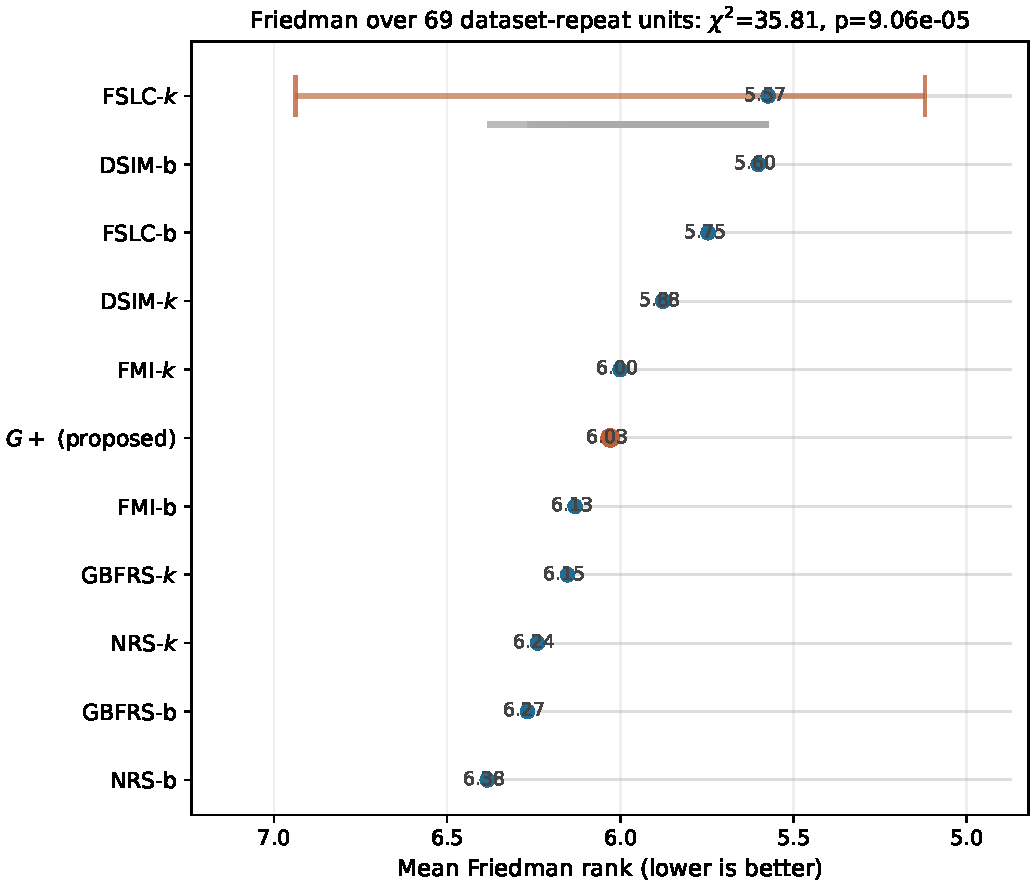
\includegraphics[width=\linewidth,height=.45\textheight,keepaspectratio]{paper_figures/expansion_cd.pdf}
	\caption{Mean Friedman ranks over the sixty-nine expansion dataset--repeat units (audit Brier; ties on guard-empty datasets receive average ranks), one row per method. The orange band is the Nemenyi critical difference (CD = 1.82) around $G+$; blue markers lie within it and are not statistically separated from $G+$.}
	\label{fig:expansion-cd}
\end{figure}


\subsection{Algorithmic Verification and Methodological Scope}
\label{subsec:logic-verification}

To confirm the operational integrity and implementation fidelity of the proposed optimization framework, we perform systematic verification across synthetic benchmark structures and delineate the methodological scope of the empirical evaluations.

\paragraph{Exact Search Verification on Synthetic Benchmark Topologies}
We benchmarked the exact branch-and-bound optimization implementation (Section~\ref{subsec:exact-search}) against exhaustive minimum-cost enumeration across $80$ synthetic non-monotone loss-dependency profiles ($m=6$ attributes). The algorithm achieved $100\%$ exact solution agreement across all evaluation scenarios. Specific stress-test configurations confirmed the algorithmic handling of critical boundary cases:
\begin{enumerate}[label=(\arabic*), leftmargin=*]
	\item \textbf{Sub-Floor Singletons:} Correct identification of highly predictive individual attributes situated below the historical dependency threshold;
	\item \textbf{Synergistic Feature Pairs:} Accurate traversal of multi-attribute interactions across non-monotonic loss plateaus via the signed predictive bridge;
	\item \textbf{Degenerate Zero-Cost Optima:} Provable convergence to the empty attribute set ($P^* = \varnothing$) when structural feature signals fail to surpass the uninformative baseline.
\end{enumerate}
These formal checks confirm that the branch pruning logic and feasibility enforcement operate in exact conformance with the theoretical minimum-cost formulation.

\paragraph{Methodological Scope and Evaluation Boundaries}
To maintain rigorous methodological transparency, we explicitly define the operational boundaries of the reported experiments:
\begin{enumerate}[label=(\arabic*), leftmargin=*]
	\item \textbf{Scoring Core Evaluation:} In Section~\ref{sec:paper-published}, competing methods are benchmarked by isolating their core representation scoring metrics within a unified, standardized evaluation pipeline. While this controls for extraneous algorithmic discrepancies (e.g., heterogeneous stopping criteria or auxiliary preprocessing), broader end-to-end pipeline comparisons under diverse downstream learners represent a valuable direction for future multi-center studies.
	\item \textbf{Scalability and Exact Optimality Gaps:} The branch-and-bound solver provides theoretical exactness for compact problem instances, but exhaustive exploration becomes computationally prohibitive on high-dimensional datasets. In large-scale real-world deployments, the guided heuristic search ($G/G+$) serves as an effective, polynomial-time surrogate, balancing feature acquisition costs against predictive loss feasibility.
\end{enumerate}